%!TEX program = xelatex

\documentclass[master,openany,electronic]{tongjithesis}
% \documentclass[%
%   master|doctor, % mandatory option
%   xetex|pdftex|dvips|dvipdfm, % optional
%   utf|gbk,
%   electronic,
%   openany|openright]{tongjithesis}

% 所有其它可能用到的包都统一放到这里了,可以根据自己的实际添加或者删除。
\usepackage{tongjiutils}
\usepackage[top=3.23cm, bottom=2.54cm, left=3.17cm, right=3.17cm]{geometry}

% 显示交叉引用的标签
%\usepackage{showkeys}

% 显示页面布局
%\usepackage{layout}

\def\myname{李勇奇}

\begin{document}

% 显示页面布局
%\layout

\graphicspath{{fig/}}

%%% 封面部分
\frontmatter
%!TEX root = ../thesis.tex

% 保密文字位置可能有问题,需要到cls文件中调整
\secretlevel{保密} \secretyear{2}

\ctitle{基于RGB-D图像的三维物体识别算法的研究与实现}
% 按照申请工学学位设计。如有其它需要,请修改相应文字。
\makeatletter
  \iftongji@doctor
    \cdegree{博士}
  \else
    \iftongji@master
      \cdegree{硕士}
    \fi
  \fi

\makeatother

\cauthor{李勇奇} % 姓名

\snumber{1531620}  % 学号

\cdepartment{电子与信息工程学院}

\cmajorfirst{工学}

\cmajorsecond{控制科学与工程}

\csupervisor{陈启军 ~ 教授}

\cassosupervisor{}
% 如果没有副指导老师或者联合指导老师,把各自{}中内容留空即可。

\ccosupervisor{}

% 日期自动生成,如果你要自己写就改这个cdate
%\cdate{\CJKdigits{\the\year}年\CJKnumber{\the\month}月}
\makeatletter
  \iftongji@doctor
    \edegree{Doctor of Philosophy}
  \else
    \iftongji@master
      \edegree{Master of Engineering}
    \fi
  \fi

\makeatother

%\cfunds{国家自然科学基金资助(项目号:XXXXXX)}

%\efunds{Supported by the Natural Science Foundation of China(No.XXXXXX)}


\etitle{3D Object Recognition and Pose Estimation \\ Based on RGB-D Images}

\eauthor{Li Yongqi}

\edepartment{College of Electronics and Information Engineering}

\emajorfirst{Engineering}%Science in

\emajorsecond{Control Science and Engineering}

\esupervisor{Prof. ~ Chen Qijun}
\eassosupervisor{}

% 这个日期也会自动生成,你要改么?
%\edate{March, 2017}

% 定义中英文摘要和关键字
\begin{cabstract}
  三维视觉是机器人感知的重要组成部分,但其目前的技术水平难以帮助机器人有效地感知周围的三维世界。随着近几年深度学习的发展,计算机视觉领域取得了巨大的发展,尤其是在2D视觉领域,2D目标的检测和分类的准确率得到了巨大的提升,但3D目标的检测并没有巨大的提升。因此,本文针对机器人目前三维感知的困难,通过参考深度学习在2D视觉上的突破,将其引入到3D视觉上来,提出了3D-MRAI算法,用于解决对3D目标的检测以及位姿的估计。

  深度信息的质量对3D目标检测以及位姿估计的准确率和精度都有至关重要的影响,因此为了获取高质量的深度信息,本文针对现有RGB-D相机的缺点,提出了对偶RGB-D相机结构,通过组合两个低价的RGB-D相机来获取高质量的深度信息,提高了相机获取深度图的填充率并且增强了深度信息的鲁棒性。

  为了能够在RGB-D图中检测出目标物体的种类以及位姿,本文提出的3D-MRAI算法分为两步,第一步在相机拍摄的三维点云中分割出目标物体点云;第二步通过点云匹配算法求解出目标的位姿。为了分割出目标物体点云,本文基于2D目标检测中的Faster R-CNN和Mask R-CNN两个算法,提出了3D Faster R-CNN和3D Mask R-CNN算法,3D Faster R-CNN和3D Mask R-CNN通过将深度图变换为HHA图,有效地利用三维信息,并结合RGB图完成对目标物体的检测,并且为了应对目标物体的各种姿态,算法还引入了Spatial Transformer结构。3D Faster R-CNN和3D Mask R-CNN相比Faster R-CNN和Mask R-CNN充分利用三维信息,对检测一些纹理较少(Textureless)的物体有着更高的准确率。为了求解目标的位姿,本文通过匹配目标物体点云和目标物体3D模型来实现,为此基于4PCS算法提出了A4PCS-ICP点云匹配算法,通过在改进4PCS算法的基础上引入ICP算法提高了匹配精度。

  本文还将所提出的3D-MRAI算法实际应用到Bin-Picking问题上,设计了一个基于3D-MARI算法的随机分拣视觉系统,所设计的系统在实验中达到了100\%的抓取成功率,并且算法的运算时间也完全满足实际应用。
\end{cabstract}

\ckeywords{RGB-D,目标检测,位姿估计,随机分拣}


\begin{eabstract}
3D vision is an important part of robot perception, but the technology of 3D vision currently is hard to help robots effectively perceive the surrounding 3D world. With the development of deep learning in recent years, tremendous development has been made in the field of computer vision. Especially in the field of 2D vision, the accuracy of 2D object detection and classification has been greatly improved, but the detection of 3D objects has not been huge Enhance. Therefore, for the difficulty of current 3D robot perception. This paper proposed a new algorithm 3D-MRAI, which introduced deep learning into 3D vision based on the breakthrough of deep learning in 2D vision. This algorithm is proposed to solve the problem of 3D object detection and pose estimation .

High-quality depth map has a great influence on the results of 3D object detection and pose estimation. To acquire high-quality depth map, a dual RGB-D camera structure is proposed to overcome the shortcomings of the existing RGB-D cameras. Dual RGB-D camera can obtain high-quality depth map by combining two low-cost RGB-D cameras, which also increases the fill rate of depth map and enhances depth value in depth map.

To detect object and estimate pose in a given RGB-D frame, 3D-MRAI algorithm proposed this paper runs in two stage. The first stage is to get the point cloud of the object from the RGB-D frame. The second stage is to estimate the object pose by point cloud matching. To segement the point cloud of the object, 3D Faster R-CNN and 3D Mask R-CNN are proposed based on two algorithm in 2D object detection: Faster R-CNN and Mask R-CNN. 3D Faster R-CNN and 3D Mask R-CNN take full advantage of depth value by converting depth map into HHA frame and detect object by combining RGB and HHA. 3D Faster R-CNN and 3D Mask R-CNN also use Spatial Transformer to detect object in arbitrary pose.  3D Faster R-CNN and 3D Mask R-CNN have higher detection accuracy when detecting textureless objects, comparing to Faster R-CNN and Mask R-CNN. In order to estimate the pose of the target, we match the 3D model of the object to the point cloud of the object. For this purpose, a new point cloud matching algorithm call A4PCS-ICP is proposed. A4PCS-ICP algorithm has higher matching accuracy by combining ICP and modified 4PCS.

  This paper also applies the proposed 3D-MRAI algorithm to solve the Bin-Picking problem. A bin-picking vision system is designed based on 3D-MARI algorithm. The designed system achieves 100\% successful picking rate, and the system's response time also fully meets the application.

\end{eabstract}

\ekeywords{RGB-D, object detection, pose estimation, Bin-Picking}

%%% Local Variables:
%%% TeX-master: "../thesis.tex"
%%% End:
\makecover

% 目录
\tableofcontents

% 符号对照表
%!TEX root = ../thesis.tex
\begin{denotation}
\item[GNU] GNU's Not Unix /'gnu:/
\item[GFDL] GNU Free Documentation License
\item[GPL] GNU General Public License
\item[FSF] Free Software Foundation
\end{denotation}


%%% 以下索引按需要选择
% 插图索引
%\listoffigures
% 表格索引
%\listoftables
% 公式索引
%\listofequations

%%% 正文
\mainmatter
\chapter{引言}
\label{chap:introduction}
本文\cite{tex}

%%% Local Variables:
%%% TeX-master: "../thesis.tex"
%%% End:
%!TEX root = ../thesis.tex
\chapter{RGB-D图像的获取与融合}
\label{chap:rgbd}

\section{3D相机现状与分析}
% @TODO: 3d相机现状

\section{RGB-D相机}
\subsection{RGB-D相机原理与结构}
RGB-D相机获取深度的原理大致可以分为三种:
\begin{itemize}
\item Structure Light
\item Time of Flight(ToF)
\item Stereo
\end{itemize}

% @TODO: 加些原理图?
Structure Light获取深度信息的原理是通过激光发射器投射带有特定编码的结构光到物体表面后,由IR Camera采集,根据采集到的光信号量的变化来计算物体的深度。举一个形象的例子,将手电筒照向墙面,手电筒离墙面越远,墙面上所形成的光斑的直径就越大,所以可以通过光斑的直径来计算手电筒距离墙面的距离。ToF获取深度信息的原理是通过专有的传感器捕捉红外光发射到接收的飞行时间来计算物体的深度。Stereo是通过双摄像头拍摄物体,再通过特征点匹配,根据三角测量原理来计算物体的深度。

三种原理的深度相机各有其特点,采用Structure Light原理的深度相机一般精度比较高,但景深比较短并且受光线影响比较大,适合室内场景;ToF原理的深度相机获取深度图的精度和分辨率一般都比较低,但帧率高,并且具有一定的抗光照性能;Stereo获取深度精度适中,帧率相对来说较低,并且需要较强的计算性能,但抗光照能力强,适合室外场景。

本文所使用的RGB-D相机是Intel的Realsense SR300相机,SR300采用的结构光的原理获取深度\footnote{此后所提到的RGB-D相机均指与SR300相机类似的采用结构光原理获取深度的RGB-D相机},其内部结构如图\ref{fig:sr300}所示。
\begin{figure}[!ht]
  \centering
  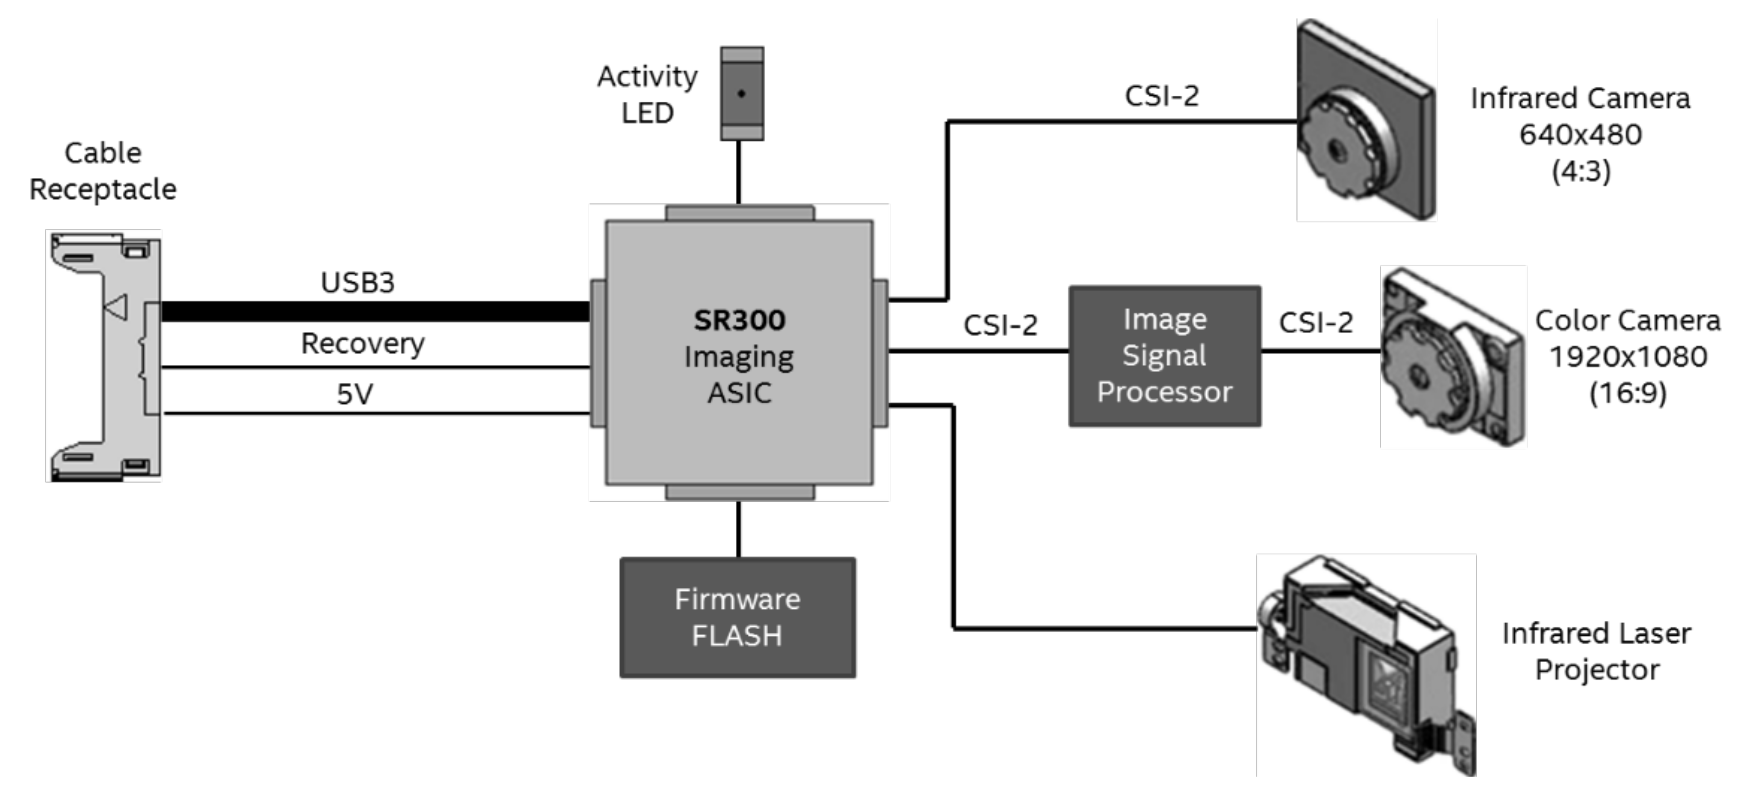
\includegraphics[width=12cm]{sr300}
  \caption{Realsense SR300内部结构图}
  \label{fig:sr300}
\end{figure}
从图\ref{fig:sr300}可以看出,SR300内部的传感器主要有彩色摄像头(Color Camera)、红外激光发射器(Infrared Laser Projector)和红外摄像头(Infrared Camera)。Color Camera是1920×1080像素的普通针孔摄像头,用来获取彩色图像;Infrared Laser Projector和Infrared Camera用来获取深度图像或者红外成像图,两种成像流程如图\ref{fig:capture_flow}所示。
\begin{figure}[!ht]
  \centering
  \subfloat[Depth Video Data Flow]{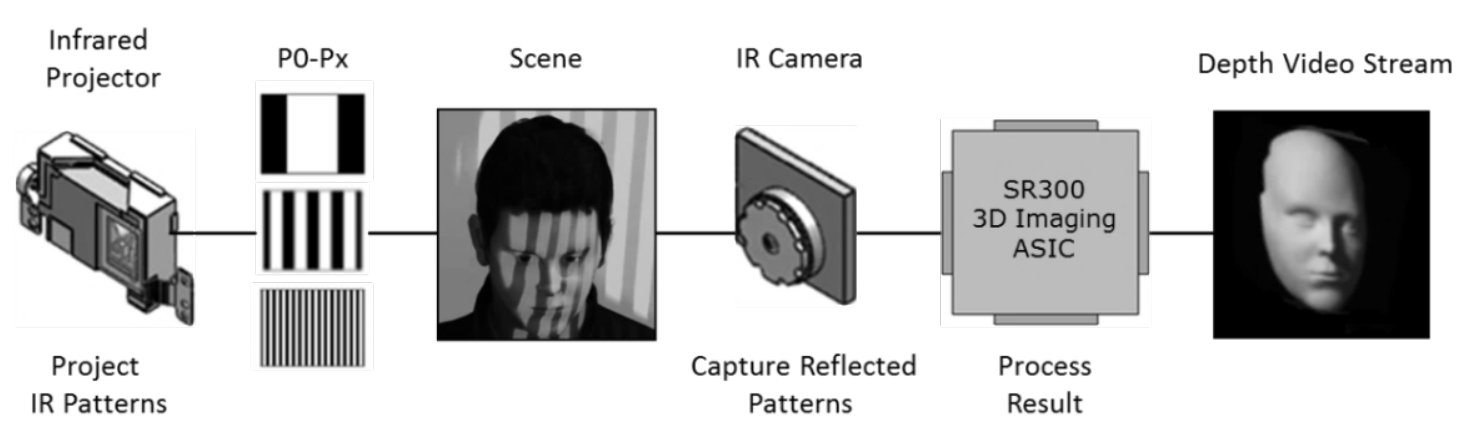
\includegraphics[width=12cm]{depth_flow}}
  \vfill
  \subfloat[IR Video Data Flow]{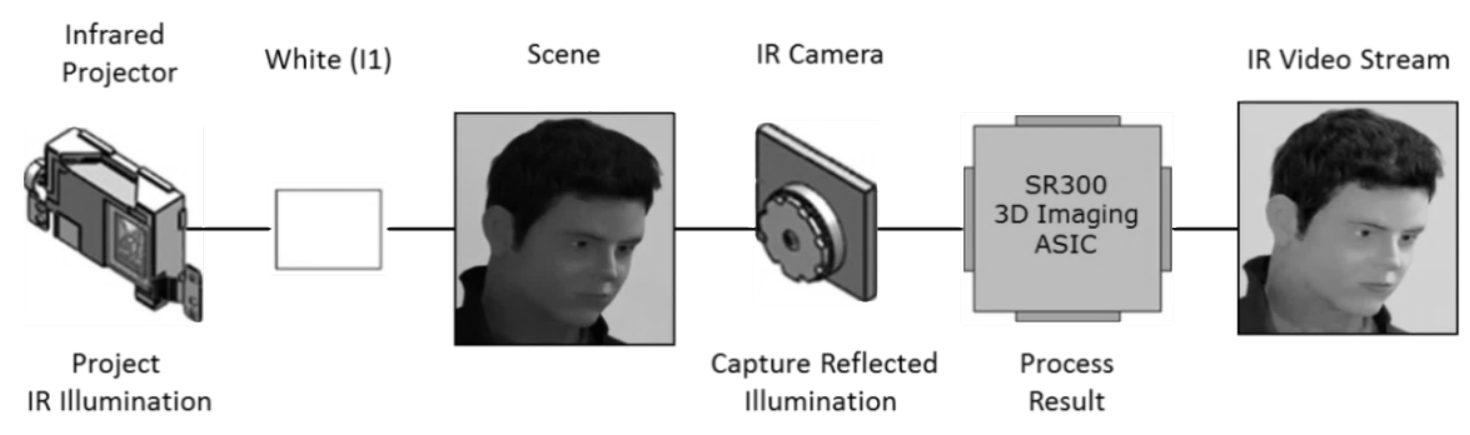
\includegraphics[width=12cm]{ir_flow}}
  \caption{Realsense SR300深度成像流程}
  \label{fig:capture_flow}
\end{figure}
其中当Infrared Laser Projector投射带有编码的结构光时,Infrared Camera可以获取深度图;当投射不带编码的红外光时,Infrared Camera可以获取红外成像图。正常使用时,往往设置Infrared Laser Projector投射带有编码的结构光来获取深度信息。因此,从RGB-D相机的使用来看,可以忽略其内部具体结构,将其看成由一个彩色摄像头和一个深度摄像头构成,其中彩色摄像获取彩色(RGB)信息,深度摄像头获取深度(depth)信息。

\subsection{RGB-D相机的数学模型}
\begin{figure}[!ht]
  \centering
  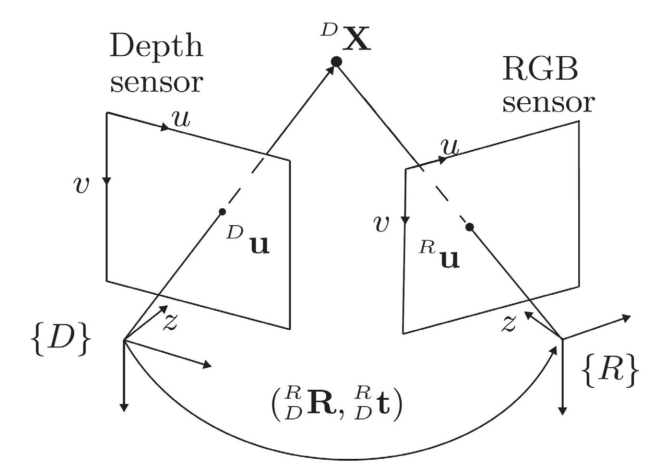
\includegraphics[width=8cm]{rgbd_model}
  \caption{RGB-D相机模型}
  \label{fig:rgbd_model}
\end{figure}
图\ref{fig:rgbd_model}展示了本文所使用的RGB-D相机的基本物理模型,其中彩色摄像头和深度摄像头都使用了针孔(pin-hole)相机模型\cite{Heikkila2000}。
先考虑普通针孔相机的模型,相机图像坐标系下一点$\bm{u}:=[u,v]^T$,对应的三维世界中的一点在相机坐标系下表示为$\bm{X}:=[x,y,z]^T$。根据针孔相机模型有:
\begin{equation}
  \label{eq:cam_model}
  z\bm{\tilde{u}} = \bm{K}\bm{X}
\end{equation}
其中$\bm{\tilde{u}}$表示$\bm{u}$的齐次变换形式,彩色相机的内参矩阵$\bm{K}$的定义如下:
\begin{equation}
  \bm{K} := \left[
    \begin{array}{ccc}
      f_u&0&u_0 \\
      0&f_v&v_0 \\
      0&0&1
    \end{array}
  \right]
\end{equation}
其中$f_u$和$f_v$分别表示彩色相机在图像坐标轴上的焦距(以像素为单位),$u_0$和$v_0$表示彩色相机光心在图像平面的投影中心。

公式\ref{eq:cam_model}还未考虑镜头的畸变,为了提高相机的精度,现引入径向畸变(radial distortion)和切向畸变(tangential distortion):
\begin{itemize}
\item 径向畸变是由相机透镜的不完善和表面曲率存在误差造成的,径向畸变的数学模型可以表示为:
  \begin{equation}
    \label{eq:radial}
    \left\{
      \begin{array}{ccc}
        \hat{x}&=&\bar{x}(1 + k_1r^2 + k_2r^4 + k_3r^6)\\
        \hat{y}&=&\bar{y}(1 + k_1r^2 + k_2r^4 + k_3r^6)\\
      \end{array}
    \right.
  \end{equation}
  其中
  \begin{align}
    \bar{x} =& x/z\\
    \bar{y} =& y/z\\
    r  =& \sqrt{\bar{x}^2 + \bar{y}^2}
  \end{align}
  $\bar{x}$,$\bar{y}$表示点$\bm{X}$在归一化平面上的坐标,$\hat{x}$,$\hat{y}$表示修正径向畸变后的的坐标,$k_1$,$k_2$,$k_3$表示径向畸变的参数。
\item 切向畸变是由于相机透镜与图像平面不平行造成的,其数字模型可以表示为:
  \begin{equation}
    \label{eq:trang}
    \left\{
      \begin{array}{ccc}
        \hat{x}&=&\bar{x} + (2p_1\bar{x}\bar{y} + p_2(r^2 + 2\bar{x}^2))\\
        \hat{y}&=&\bar{y} + (p_1(r^2 + 2\bar{y}^2) + 2p_2\bar{x}\bar{y})\\
      \end{array}
    \right.
  \end{equation}
  其中$p_1$,$p_2$是切向畸变的参数。
\item 结合公式\ref{eq:radial}和\ref{eq:trang}可以得到修正径向畸变和切向畸变的Brown–Conrady模型\cite{Brown1966}:
  \begin{equation}
    \label{eq:dist}
    \left\{
      \begin{array}{ccc}
        \hat{x}&=&\bar{x}(1 + k_1r^2 + k_2r^4 + k_3r^6) + (2p_1\bar{x}\bar{y} + p_2(r^2 + 2\bar{x}^2))\\
        \hat{y}&=&\bar{y}(1 + k_1r^2 + k_2r^4 + k_3r^6) + (p_1(r^2 + 2\bar{y}^2) + 2p_2\bar{x}\bar{y})\\
      \end{array}
    \right.
  \end{equation}
\end{itemize}
通过以上分析,根据公式\ref{eq:cam_model}和\ref{eq:dist}可以推导出带有畸变的针孔相机模型:
\begin{equation}
  \label{eq:dist_cam_model}
  \left\{
    \begin{array}{ccc}
      u&=&f_u(\bar{x}(1 + k_1r^2 + k_2r^4 + k_3r^6) + (2p_1\bar{x}\bar{y} + p_2(r^2 + 2\bar{x}^2))) + u_0\\
      v&=&f_v(\bar{y}(1 + k_1r^2 + k_2r^4 + k_3r^6) + (p_1(r^2 + 2\bar{y}^2) + 2p_2\bar{x}\bar{y})) + v_0
    \end{array}
  \right.
\end{equation}
为方便起见,记$\bm{d}:=[k_1,k_2,p_1,p_2,k_3]^T$,定义函数
\begin{equation}
  f_{undist}(\bm{d}, \bm{X}):=\left[
    \begin{array}{ccc}
      \bar{x}(1 + k_1r^2 + k_2r^4 + k_3r^6) + (2p_1\bar{x}\bar{y} + p_2(r^2 + 2\bar{x}^2))\\
      \bar{y}(1 + k_1r^2 + k_2r^4 + k_3r^6) + (p_1(r^2 + 2\bar{y}^2) + 2p_2\bar{x}\bar{y})\\
    \end{array}
  \right]
\end{equation}
\begin{equation}
  \tilde{f}_{undist}(\bm{d}, \bm{X}):=\left[
    \begin{array}{c}
      f_{undist}(\bm{d}, \bm{X})\\
      1
    \end{array}
  \right]
\end{equation}
则公式\ref{eq:dist_cam_model}可简化为:
\begin{equation}
  \tilde{\bm{u}} = \bm{K}\cdot \tilde{f}_{undist}(\bm{d}, \bm{X})
\end{equation}
其中需要标定的参数有相机内参矩阵$\bm{K}$(包含未知参数$f_u$,$f_v$,$u_0$,$v_0$)以及畸变参数$\bm{d}$(包含未知参数$k_1$,$k_2$,$p_1$,$p_2$,$k_3$),共9个参数。

明确了针孔相机的数学模型后,很容易推出SR300的相机模型:
\begin{equation}
  \label{eq:rgbd_cam_model}
  \left\{
    \begin{array}{ccc}
      \tensor*[^R]{\tilde{\bm{u}}}{}&=&\tensor*[^R]{\bm{K}}{}\cdot \tilde{f}_{undist}(\tensor*[^R]{\bm{d}}{},\tensor*[^R]{\bm{X}}{})\\
      \tensor*[^D]{\tilde{\bm{u}}}{}&=&\tensor*[^D]{\bm{K}}{}\cdot \tilde{f}_{undist}(\tensor*[^D]{\bm{d}}{},\tensor*[^D]{\bm{X}}{})\\
      \tensor*[^R]{\bm{X}}{} &=& \tensor*[^R_D]{\,\bm{R}}{}\tensor*[^D]{\bm{X}}{} + \tensor*[^R_D]{\,\bm{t}}{}
    \end{array}
  \right.
\end{equation}
其中左上标$\{R\}$表示SR300相机中的彩色相机(RGB),$\{D\}$表示SR300相机中的深度相机(Depth),$\tensor*[^R_D]{\,\bm{R}}{}$和$\tensor*[^R_D]{\,\bm{t}}{}$表示了彩色相机坐标系和深度相机坐标系之间的齐次变换关系。

\subsection{RGB-D相机的标定流程}
\label{sec:rgb-d_calibration}
根据上文所述的RGB-D相机的结构及数学模型,RGB-D相机的标定主要涉及到彩色摄像头内参和畸变的标定,深度摄像头内参和畸变的标定,以及彩色摄像头和深度摄像头之间位姿变换的标定。由于RGB-D相机是一种较为新颖的相机,所以市面上基本上没有较为成熟通用的标定RGB-D相机的方法以及对应的工具。因此本文针对所使用的Realsense SR300相机,设计了一套标定方法。

根据公式\ref{eq:rgbd_cam_model}可知相机需要标定的参数有彩色相机内参和畸变参数9个,深度相机内参和畸变参数9个,彩色相机和深度相机之间的位姿关系6个,一共24个参数。一起标定这24个参数理论上是相当困难的,考虑到普通针孔相机的标定技术已经相当成熟(如张正友的棋盘格标定\cite{Zhang2002},以及RGB-D相机中彩色相机和深度相机的解耦性,因此所设计的标定方法分为三步:
\begin{enumerate}[Step 1]
\item 标定彩色相机内参以及畸变参数
\item 标定深度相机内参以及畸变参数
\item 标定彩色相机和深度相机之间的齐次变换关系
\end{enumerate}

步骤1标定彩色相机内参以及畸变参数相对来说比较简单,主要参考文献\cite{Zhang2002},但所使用的标定板是不对称圆盘标定板(Asymmetrical Circle Board),如图\ref{fig:circle_board}是$4\times 11$的不对称圆盘标定板。
\begin{figure}[!ht]
  \centering
  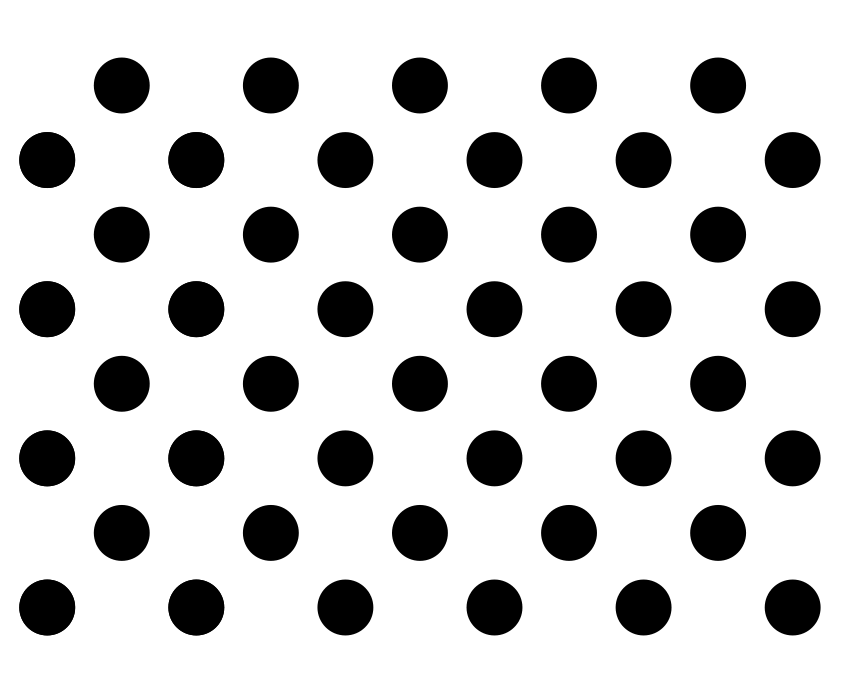
\includegraphics[width=10cm]{circle_board}
  \caption{Asymmetrical Circle Board}
  \label{fig:circle_board}
\end{figure}
使用圆盘标定板而非棋盘格标定板的原因是圆盘相对于棋盘格有更高的检测精度,在某些情况下可以达到0.1到0.01像素的亚像素精度,当然代价是相比计算棋盘格的角点,计算椭圆(圆形经过投影变换后退化为椭圆)的中心会涉及到较为复杂的数学运算,这也是为什么工业上大多使用圆盘作为标定板的原因。

步骤2标定深度相机内参以及畸变参数的方法和步骤1类似,区别在于深度相机并不能直接获得颜色信息,因此也不能直接检测图\ref{fig:circle_board}所示的标定板。但是,幸运的是,根据前文所述的SR300深度相机的原理,其本质上也是个普通的针孔相机,只不过在其镜头上加上了滤波片,可以认为其只对红外光成像。因此,只要使用图\ref{fig:capture_flow}中的红外成像模式获取红外成像图,在红外成像图上检测标定板。如图\ref{fig:circle_on_ir}所示,在红外成像图中检测出了标定板。
\begin{figure}[!ht]
  \centering
  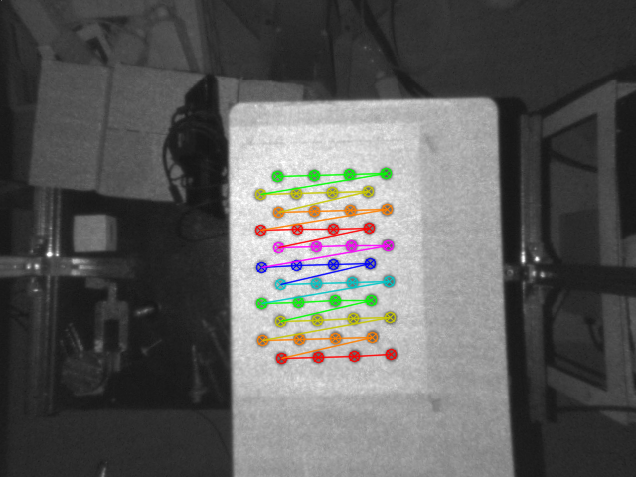
\includegraphics[width=12cm]{circle_on_ir}
  \caption{红外成像图中检测标定板}
  \label{fig:circle_on_ir}
\end{figure}

步骤3标定彩色相机和深度相机之间的齐次变换关系需要依赖于步骤1和步骤2中标定出的彩色相机和深度相机的内参和畸变参数,具体做法是将标定板放在彩色相机和深度相机下,使彩色相机和深度相机能够同时检测到标定板,然后分别根据各自的内参和畸变参数计算出标定板的位姿$\tensor*[^R_B]{\bm{H}}{}$和$\tensor*[^D_B]{\bm{H}}{}$,其中$\tensor*[^R_B]{\bm{H}}{}$是$4\times 4$的齐次变换矩阵,表示标定板在彩色相机坐标系下的位姿,也是彩色相机坐标系变换到标定板坐标系的齐次变换矩阵;$\tensor*[^D_B]{\bm{H}}{}$也是$4\times 4$的齐次变换矩阵,表示标定板在深度相机坐标系下的位姿,也是深度相机坐标系变换到标定板坐标系的齐次变换矩阵。从而所要求的彩色相机坐标系变换到深度相机坐标系的齐次变换矩阵为:
\begin{equation}
  \tensor*[^R_D]{\bm{H}}{} = \tensor*[^R_B]{\bm{H}}{}\tensor*[^D_B]{\bm{H}}{^{-1}}
\end{equation}
其中
\begin{equation}
  \tensor*[^R_D]{\bm{H}}{} := \left[
    \begin{array}{cc}
      \tensor*[^R_D]{\bm{R}}{}& \tensor*[^R_D]{\bm{t}}{}\\
      \bm{0}_{1\times 3}&1
    \end{array}
\right]
\end{equation}
当然,实际标定时,往往会采取多组$\tensor*[^R_B]{\bm{H}}{}$和$\tensor*[^D_B]{\bm{H}}{}$来提高标定的精度。

\section{对偶RGB-D相机}
使用SR300相机时,发现相机在某些情况下,对一些反光的物体的深度图有严重的缺失,具体如图\ref{fig:depth_missing}所示。
\begin{figure}[!ht]
  \centering
  \subfloat[彩色图]{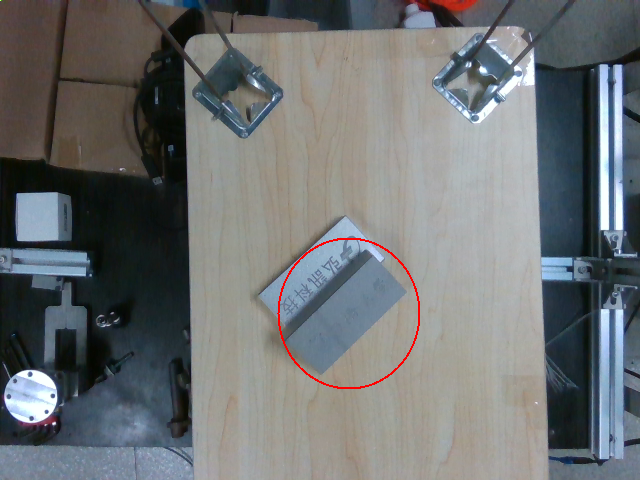
\includegraphics[width=7cm]{left_color}}
  \hfill
  \subfloat[深度图]{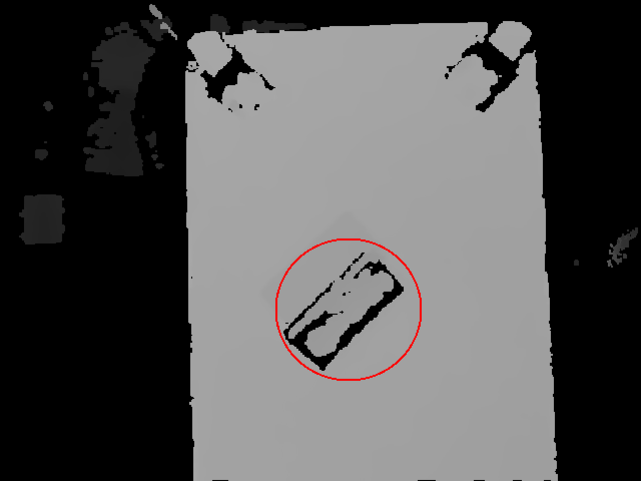
\includegraphics[width=7cm]{left_depth}}
  \caption{SR300采集的物体深度信息部分缺失情况下的深度图}
  \label{fig:depth_missing}
\end{figure}
经过实验,发现这种缺失情况的出现和拍摄的角度以及光线有关,因此本文提出一种组合相机对偶RGB-D相机(Dual RGB-D Camera)。

\subsection{对偶RGB-D相机原理与结构}
对偶RGB-D相机在原RGB-D相机的基础上,通过增加一个与原相机呈180度夹角的RGB-D相机构成,实际物理结构如图\ref{fig:dual_rgbd}所示。
\begin{figure}[!ht]
  \centering
  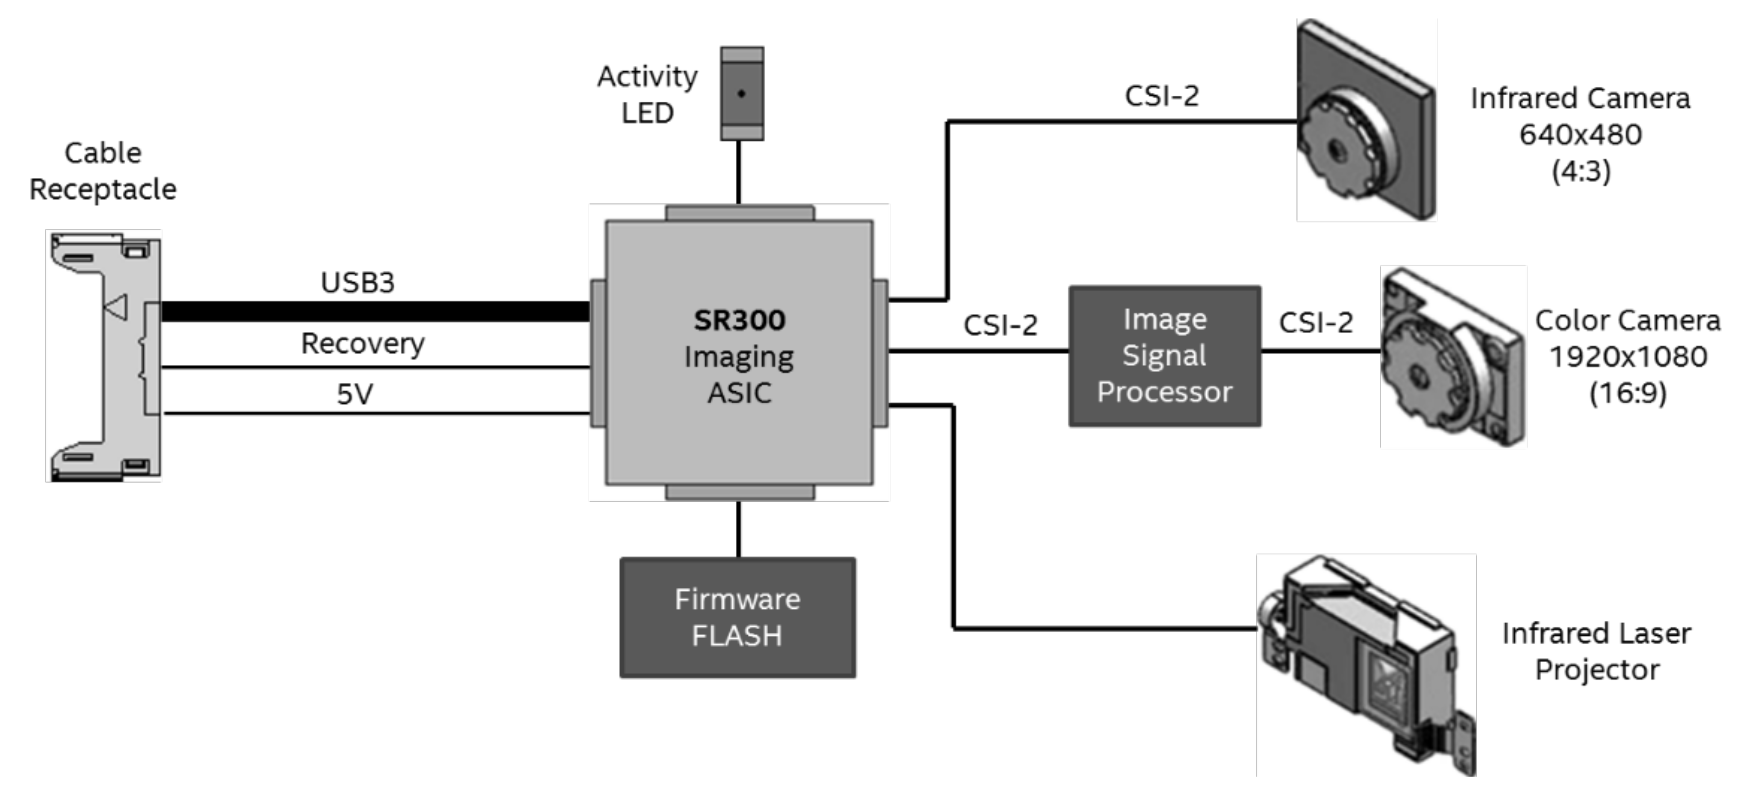
\includegraphics[width=6cm]{dual_rgbd}
  \caption{对偶RGB-D相机实际物理结构}
  \label{fig:dual_rgbd}
\end{figure}

对于对偶RGB-D相机,当其中一个相机深度图出现严重缺失时,另外一个相机的深度图往往不会在相同的地方深度信息出现严重的缺失,如图\ref{fig:dual_rgbd_depth}所示\footnote{实际下相机采集的图像与上相机采集的图像相差了180度,为了方便起见,都将下相机采集的图像旋转了180度}
,有效的避免了单个RGB-D相机某些情况下深度信息严重缺失的情况。
\begin{figure}[!ht]
  \centering
  \subfloat[上相机采集的深度图]{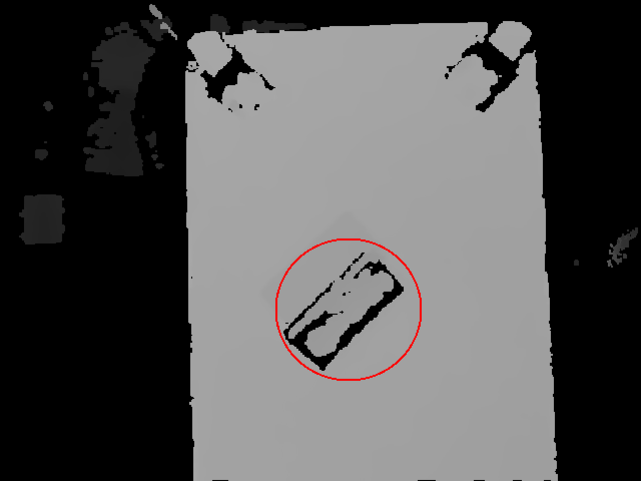
\includegraphics[width=7cm]{left_depth}}
  \hfill
  \subfloat[下相机采集的深度图]{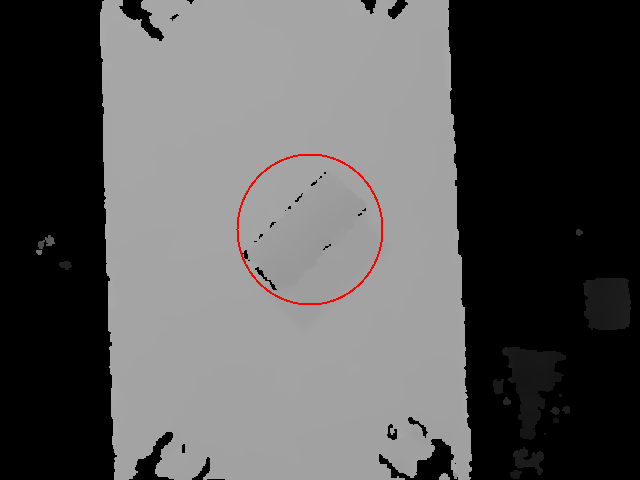
\includegraphics[width=7cm, angle=180, origin=c]{right_depth}}
  \caption{对偶RGB-D相机采集的左右两张深度图}
  \label{fig:dual_rgbd_depth}
\end{figure}

除此之外,对偶RGB-D相机还可以利用两个相机的彩色图构成双目,生成第三张深度图,从而通过设计的深度的融合算法将三张深度图融合成为一张质量更高的深度图,其内部原理如图\ref{fig:dual_rgbd_struct}所示。
\begin{figure}[!ht]
  \centering
  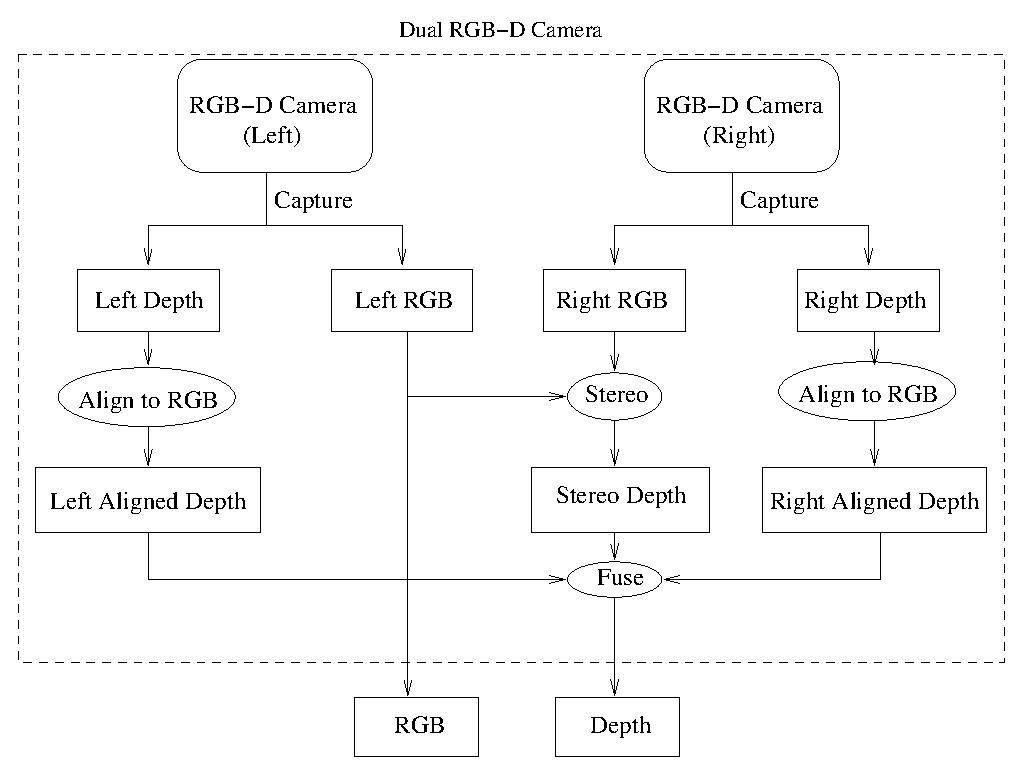
\includegraphics[width=14cm]{dual_rgbd_struct}
  \caption{对偶RGB-D相机内部原理图}
  \label{fig:dual_rgbd_struct}
\end{figure}

从外部使用来看,对偶RGB-D相机也输出一张彩色图、一张深度图。输出的彩色图就是从上相机采集到的彩色图;输出的深度图是由三张深度图融合而成,并且与输出的彩色图相对齐,对齐的意思是彩色图和深度图相同图像坐标下的颜色信息和深度信息对应的实际物理世界中相同的一点,对齐的意义在于方便后续的一些图像处理的算法。

从内部实现来看,主要涉及到三个部分:
\begin{itemize}
\item 将深度图与输出的彩色图对齐(Align to RGB)
\item 利用上相机采集的彩色图和下相机采集的彩色图,通过双目匹配算法形成一张新的深度图
\item 融合上相机对齐后的深度图、下相机对齐后的深度图和双目匹配得到的深度图
\end{itemize}
将深度图与彩色图对齐,相对来讲实现还是比较简单的,对齐深度图的具体流程如算法\ref{alg:align}所示。
\begin{algorithm}[!ht]
  \caption{Align Depth Frame}
  \label{alg:align}
  \KwIn{Raw Depth Frame $Raw\_D_{dh\times dw}$}
  \KwOut{Aligned Depth Frame $Aligned\_D_{ch\times cw}$}
  \For {p in $Aligned\_D$} {
    $p = 0$
  }
  \For {dy = 1; dy <= dh; ++dy} {
    \For {dx = 1; dx <= dw; ++dx} {
      通过深度相机内参将点$(dx, dy)$反投影到三维空间一点$\tensor*[^D]{\bm{X}}{}$\;
      坐标变换$\tensor*[^R]{\bm{X}}{} = \tensor*[^R_D]{\bm{R}}{}\tensor*[^D]{\bm{X}}{} + \tensor*[^R_D]{\bm{t}}{}$\;
      通过彩色相机内参将点$\tensor*[^R]{\bm{X}}{}$投影变换到彩色图像坐标系下一点$(cx, cy)$\;
      \If {cx in $(0, cw]$ and cy in $(0, ch]$} {
        $Aligned\_D(cx, cy) = Raw\_D(dx, dy)$\;
      }
    }
  }
\end{algorithm}
算法\ref{alg:align}主要将深度图中每个点的图像坐标利用该点的深度信息反投影变换到实际三维空间中一点,然后将该点坐标变换到彩色相机坐标系下,最后通过彩色相机的内参将该点在彩色相机坐标系下的三维坐标投影变换到彩色图像上的二维坐标。实际对齐三张深度图时,对于上相机深度图对齐到上相机彩色图,需要分别知道上相机深度相机和彩色相机的内参和畸变参数以及深度相机与彩色相机之间的齐次变换关系(通过相机标定这些参数都可以得到);双目匹配得到的深度图理论上可以有两张,一张与上相机校准后的彩色图像对齐,另一张与下相机校准后的彩色图像对齐,简单起见,选择与上相机对齐的深度图,然后通过上相机校准所使用的旋转矩阵的逆矩阵即可得到与原上相机彩色图像对齐的深度图;对齐下相机到上相机彩色图,除了要知道下相机标定的参数外,还需要知道下相机与上相机之间的齐次变换关系(通过对偶RGB-D相机的标定得到)。

利用上下相机采集到的两张彩色图获取深度信息主要分为三步:
\begin{itemize}
\item 分别对两张原始图像进行校准
\item 在校准后的两张图像上通过匹配算法得到视差图
\item 通过视差图获取深度图
\end{itemize}
对两张原始图像进行校准主要通过双目相机的标定实现,使得校准后的两张图像的极线对齐,如图\ref{fig:stereo_images}所示,
\begin{figure}[!ht]
  \centering
  \subfloat[上相机原始图像]{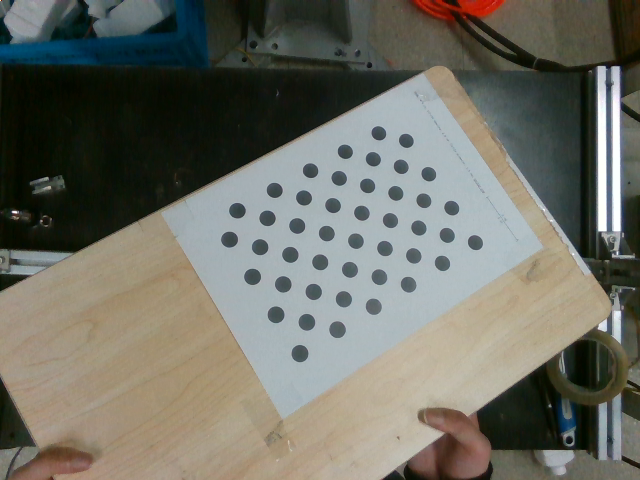
\includegraphics[width=7cm]{left_raw_image}}
  \hfill
  \subfloat[上相机校准后图像]{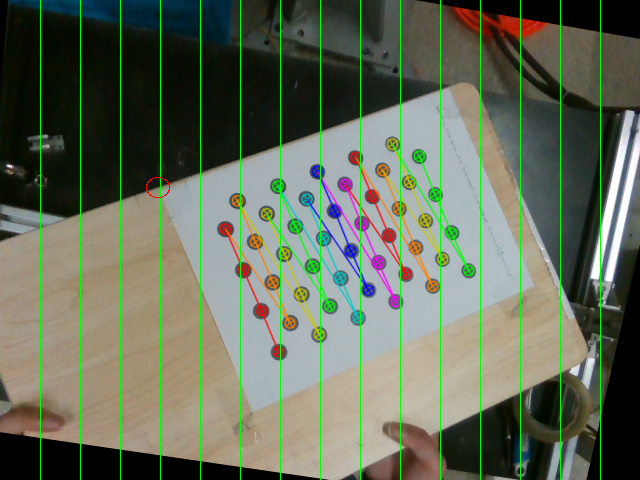
\includegraphics[width=7cm]{left_rectified_image}}
  \vfill
  \subfloat[下相机原始图像]{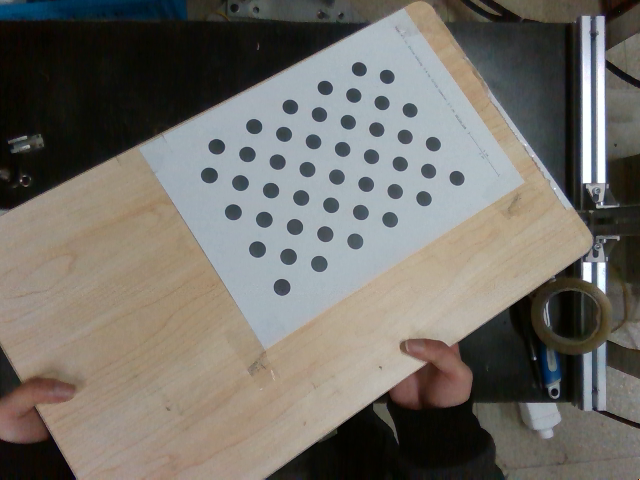
\includegraphics[width=7cm]{right_raw_image}}
  \hfill
  \subfloat[下相机校准后图像]{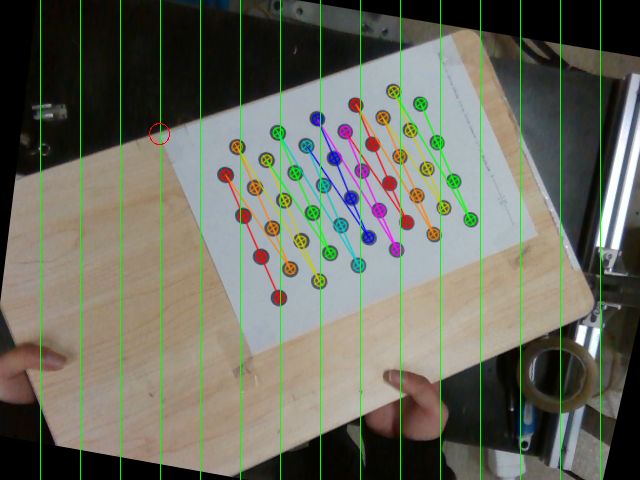
\includegraphics[width=7cm]{right_rectified_image}}
  \caption{双目相机原始图像和校准后图像}
  \label{fig:stereo_images}
\end{figure}
其中绿色的直线便是图像对齐后的部分极线,可以看出校准后的图像的对应点都分布在对齐的极线上(如图中用红色圈出的一对对应点所示),这样使得双目的匹配算法的搜索从二维缩小到了一维,只需要在极线上找对应点即可,能更快更稳定地在两张图中找到对应点。双目匹配算法使用的是ELSA算法\cite{Geiger2010},通过ELSA算法可以从两张校准后彩色图像上得到对应的视差图,视差图到深度图的变化可以通过公式\ref{eq:reprojection}得到:
\begin{equation}
  \label{eq:reprojection}
  z = \frac{\prescript{\{T,\,R\}}{}{f}B}{-(\prescript{\{T,\,R\}}{}{v_0}-\prescript{\{B,\,R\}}{}{v_0}) + \prescript{\{T,\,R\}}{}{d}}
\end{equation}
其中上标\{$T,R$\}(Top,RGB)表示上相机的RGB摄像头,\{$B,R$\}(Bottom,RGB)表示下相机的RGB摄像头,$B$表示基线长度,$\prescript{\{T,\,R\}}{}{d}$表示视差。一般地,会人为地校准过程中使得$\prescript{\{T,\,R\}}{}{v_0}-\prescript{\{B,\,R\}}{}{v_0}=0$,从而公式\ref{eq:reprojection}可以简化为:
\begin{equation}
  \label{eq:reprojection_simple}
  z = \frac{\prescript{\{T,\,R\}}{}{f}B}{\prescript{\{T,\,R\}}{}{d}}
\end{equation}

融合上相机对齐后的深度图、下相机对齐后的深度图以及双目匹配得到的深度这三张深度图的算法首先做的是分别对这三张深度图进行预处理,填补一些深度缺失的像素,因为对齐后的深度图和双目匹配得到的深度图深度信息都有细微的缺失,填补深度信息缺失的方法如算法\ref{alg:fill_hole}所示。
\begin{algorithm}[!ht]
  \caption{Fill Holes in Depth Frame}
  \label{alg:fill_hole}
  \KwIn{Depth Frame $D_{h\times w}$}
  \KwOut{Filled Depth Frame $FD_{h\times w}$}
  \For {y = 1; y <= h; ++y} {
    \For {x = 1; x <=w ; ++x} {
      \If {valid($D_{x,y}$)} {
        $FD_{x,y} = D_{x,y}$\;
      } \Else {
        $FD_{x,y}$= NAN\;
        bool leftTop = valid($D_{x-1, y-1}$) or valid($D_{x, y-1}$) or valid($D_{x-1, y}$)\;
        bool leftBottom = valid($D_{x-1, y+1}$) or valid($D_{x, y+1}$) or valid($D_{x-1, y}$)\;
        bool rightTop = valid($D_{x+1, y-1}$) or valid($D_{x, y-1}$) or valid($D_{x+1, y}$)\;
        bool rightBottom = valid($D_{x+1, y+1}$) or valid($D_{x, y+1}$) or valid($D_{x+1, y}$)\;
        \If {leftTop and leftBottom and rightTop and rightBottom} {
          validPoints = \{\}\;
          \For {dy = -1; dy <=1; ++dy} {
            \For {dx = -1; dx <=1; ++dx} {
              \If {valid($D_{dx, dy}$)} {
                push back $D_{x, y}$ to validPoints\;
              }
            }
          }
          \If {max(validPoints) - min(validPoints) < 0.05} {
            $FD_{x,y}$= mean(validPoints)\;
          }
        }
      }
    }
  }
\end{algorithm}
算法\ref{alg:fill_hole}主要实现对于深度缺失的点,将检查其周围的深度信息,当其四个角上都有有效的深度信息时,并且周围有效深度信息的极值小于一定阈值时,会用周围有效深度信息的均值填充该缺失的点。实际的效果如图\ref{fig:fill_hole}所示。
\begin{figure}[!ht]
  \centering
  % @TODO: fill hole 效果图
  \caption{填补深度信息缺失算法效果图}
  \label{fig:fill_hole}
\end{figure}
分别对深度图进行预处理后,将会对三张深度图进行线性叠加得到最终的深度图,基本叠加的公式如\ref{eq:linear}所示。
\begin{equation}
  \label{eq:linear}
  d_{fuse} = \frac{w_1d_{left} + w_2d_{right}+w_3d_{stereo}}{w_1+w_2+w_3}
\end{equation}
其中$w_1,w_2,w_3$分别表示上相机深度、下相机深度以及双目匹配深度的权重,SR300相机得到深度的精度比双目计算得到的深度要高,所以实际使用时$w_1,w_2$要比$w_3$大许多。融合三张深度图的理论相对简单,但实际上,三张深度图的深度信息并非都会永远有效,因此根据实际情况实际的融合算法如\ref{alg:fuse}所示。
\begin{algorithm}[!ht]
  \caption{Fuse Depth Frames}
  \label{alg:fuse}
  \KwIn{leftDepth, rightDepth, stereoDepth}
  \KwOut{fuseDepth}
  Initialize w1,w2,w3\;
  \For {(d1,d2,d3,d4) in (leftDepth, rightDepth, stereoDepth, fuseDepth)} {
    validDepth = [], validWeight = []\;
    \For {i = 1 to 3} {
      \If {di is valid} {
        push back di to validDepth, wi to validWeight\;
      }
    }
    \If {size of validDepth == 0} {
      d4 = NAN\;
    } \ElseIf {size of validDepth == 1} {
      d4 = validDepth[1]\;
    } \ElseIf {size of validDepth == 2 } {
      \If {extremum of validDepth < 0.03} {
        d4 = validDepth $\cdot$ validWeight / sum of validWeight\;
      } \Else {
        d4 = NAN\;
      }
    } \Else {
      mediumDepth = medium(validDepth)\;
      d4 = 0, sum = 0\;
      \For {(d,w) in (validDepth, validWeight)} {
        \If {abs(d-mediumDepth) < 0.03} {
          d4 += d*w\;
          sum += w\;
        }
      }
      \If {sum > 0} {
        d4 = d4 / sum\;
      } \Else {
        d4 = NAN\;
      }
    }
  }
\end{algorithm}
算法\ref{alg:fuse}不仅考虑了深度缺失的情况,对于深度信息差值过大的情况也进行了处理。实际处理的效果如图\ref{fig:fuse}所示。
\begin{figure}[!ht]
  \centering
  % @TODO 深度融合算法效果图
  \caption{深度融合算法效果图}
  \label{fig:fuse}
\end{figure}

\subsection{对偶RGB-D相机的标定流程}
对偶RGB-D相机的标定流程可以分为三步:
\begin{enumerate}[Step 1]
\item 分别标定好单个RGB-D相机
\item 标定出两个彩色相机之间的齐次变换关系
\item 标定出矫正彩色图像的旋转矩阵以及矫正后图像的投影矩阵
\end{enumerate}
单个RGB-D相机的标定在\ref{sec:rgb-d_calibration}小节中已经详细叙述过了,分别标定完单个RGB-D相机后,后面的步骤其实就等价于双目标定了。双目的几何结构如图\ref{fig:stereo}所示,
\begin{figure}[!ht]
  \centering
  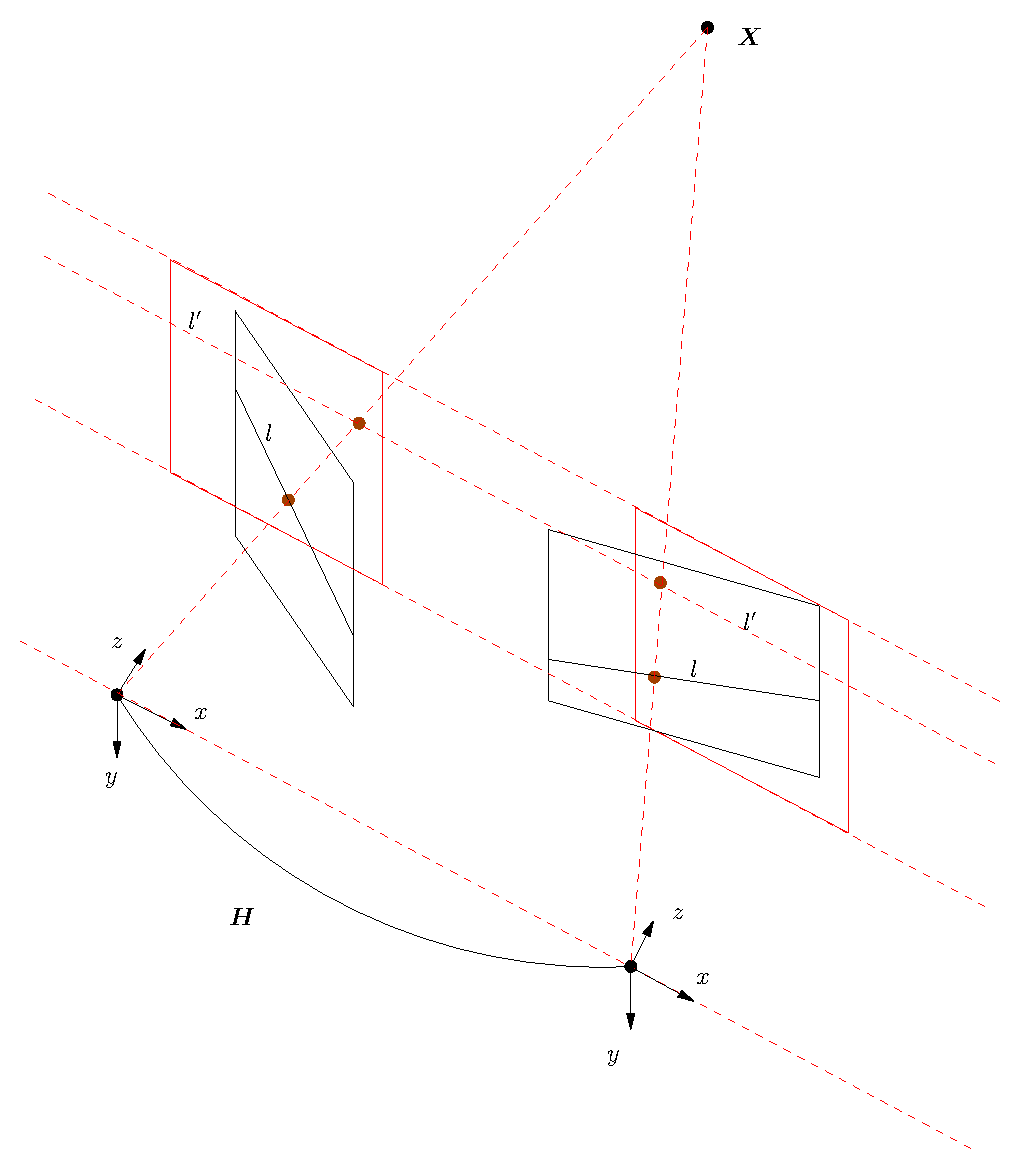
\includegraphics[width=14cm]{stereo}
  \caption{双目几何结构}
  \label{fig:stereo}
\end{figure}
标定出两个彩色相机之间的齐次变换关系,即图\ref{fig:stereo}中的$H$,简单地可以通过8点法\cite{Sur2008}先求出基础矩阵(Fundamental Matrix)$F$,即所谓的“弱标定”,然后根据相机的内参矩阵可求得本质矩阵(Essential Matrix)$E$:
\begin{equation}
  E = K^{T}FK'
\end{equation}
其中$K$和$K'$分别是两个相机的内参矩阵。求得本质矩阵后可以通过奇异值分解求得齐次变换矩阵的旋转矩阵$R$和平移向量$T$:
\begin{equation}
  \left\{\begin{array}{ccc}
    E &=& U\Sigma V^T \\
    R &=& U\bm{R}_Z^T(\frac{\pi}{2})V^T \\
    \left[T\right]_{\times} &=& U\bm{R}_Z^T(\frac{\pi}{2})\Sigma U^T
  \end{array}
  \right.
\end{equation}
其中$\bm{R}_Z(\theta)$表示绕$Z$轴旋转$\theta$角的旋转矩阵,$\left[T\right]_{\times}$的定义如下:
\begin{equation}
  \left[T\right]_{\times} = \left[
    \begin{array}{ccc}
      0&-T_z&T_y\\
      T_z&0&-T_x \\
      -T_y&T_x&0
    \end{array}
  \right]
\end{equation}
矫正彩色图像的旋转矩阵会将图\ref{fig:stereo}中黑色线框的图像平面变换到红色线框的图像平面上,使得对应点在两张图像的同一条极线上。矫正彩色图像的旋转矩阵的计算参考文献\cite{Loop2001},此步标定完最终可以得到:
\begin{itemize}
\item 两个相机的矫正旋转矩阵$R_1$,$R_2$
\item 两个矫正坐标系下的投影矩阵$P_1$,$P_2$
\item 主相机\footnote{另外一个相机的投影变换矩阵也可以得到,但没有必要。}的投影变换矩阵$Q$
\end{itemize}
其中
\begin{equation}
  Q = \left[
    \begin{array}{cccc}
      1&0&0&-u_0 \\
       0&1&0&-v_0 \\
       0&0&0&f \\
       0&0&1/B&0
    \end{array}
    \right]
\end{equation}
包含了公式\ref{eq:reprojection_simple}由视差计算深度的所有参数。

\section{RGB-D相机精度测量实验}
% @TODO: 精度测量实验

\section{本章小结}
% @TODO: 本章小结

%!TEX root = ../thesis.tex
\chapter{基于RGB-D图像的目标检测算法}
\label{chap:detector}
本章主要介绍所提出的两种基于RGB-D图像的目标检测算法3D Faster R-CNN和3D Mask R-CNN。3D Faster R-CNN是在Faster R-CNN\cite{Ren}的基础上,通过引入深度图以解决单从RGB图难以检测缺少纹理物体(Textureless Object)的问题,并且还引入了Spatial Transformer结构使得提取的特征具有旋转不变性。由于3D Faster R-CNN目标检测的结果是框出目标的Bounding Box,因此使得一些框住细长目标的Bounding Box内大部分像素并不属于该目标,这就使得后面的点云匹配算法难以得到满意的结果。因此3D Mask R-CNN根据Mask R-CNN\cite{He2017}对Faster R-CNN的改进思路,对3D Faster R-CNN进行了改进,使得其不仅能得到目标的Bounding Box,还能得到目标的Mask(可以知道Bounding Box内属于检测目标的像素),大大减少了后续匹配算法的难度。

\section{3D Faster R-CNN}
相比于Faster R-CNN,本文所提出的3D Faster R-CNN主要增加对深度信息的处理和Spatial Transformer,分别用于解决Faster R-CNN在实际应用时所不能解决的问题:
\begin{itemize}
\item 难以检测出缺少纹理的物体
\item 对物体的旋转敏感,提取的特征不具有旋转不变性
\end{itemize}

对于缺少纹理的物体,单从RGB图中很难检测出目标,这是一个很显然的问题,但是现在我们可以从对偶RGB-D相机中获取深度图,对于纹理少的物体,可以从深度图中提取特征检测出目标,所以现在的关键问题是如何从深度图中提取特征,并结合到Faster R-CNN中,本文所提出的方法是将深度图转换到HHA,然后再使用CNN提取特征,具体后文会详细介绍。

Faster R-CNN对于物体旋转敏感的问题,归根到底是因为CNN所提取的特征不具有旋转不变性,实际出现这种问题的情况,如图\ref{fig:cat}所示,
\begin{figure}[!ht]
  \centering
  \subfloat[检测旋转前的图片]{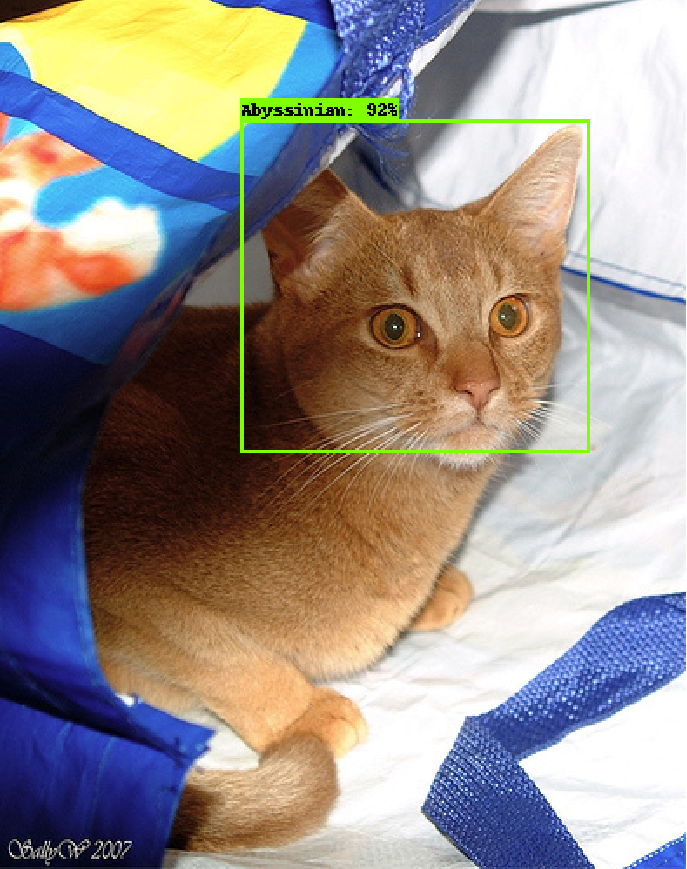
\includegraphics[width=4cm]{cat_up}}
  \hskip1em
  \subfloat[检测旋转后的图片]{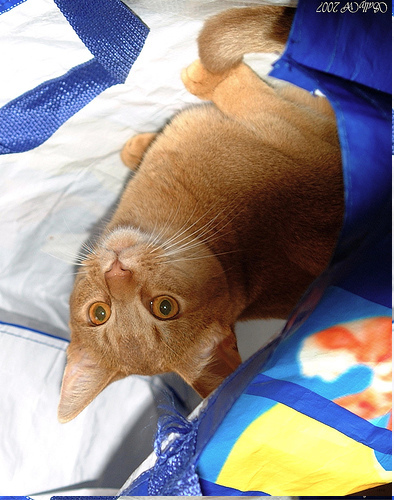
\includegraphics[width=4cm]{cat_down}}
  \caption{Faster R-CNN检测识别宠物猫示例}
  \label{fig:cat}
\end{figure}
其中图(b)只是将图(a)旋转了180度,由于CNN所提取的特征不具有旋转不变性,并且训练所实验的图片中的宠物都是头朝上的,即使图(a)在训练集中,将其旋转180度后,也无法从中检测出目标来。解决这个问题有两个思路:
\begin{itemize}
\item Data Augmentation
\item Spatial Transformer
\end{itemize}
Data Augmentation是通过对训练集中的图片进行旋转以获取不同角度的图片,通过这种方式增大数据集从而使得最终训练得到的模型对各种角度的图片都能识别;Spatial Transformer是一种特殊的网络结构,本文所使用的就这种方式,后文会详细介绍。

\subsection{HHA}

\subsection{Faster RCNN}

\subsection{Spatial Transformer}


\section{3D Mask RCNN}

\section{目标检测实验}

\section{本章小结}


\chapter{基于4PCS的点云匹配算法}
\label{chap:matcher}
本章主要介绍为了估计目标的位姿所提出的一种基于4PCS的点云匹配算法A4PCS-ICP(Angle-fixed-4PCS-ICP),A4PCS-ICP主要基于全局匹配算法4PCS\cite{aiger20084}和局部匹配算法ICP\cite{besl1992method}。为了详细介绍A4PCS-ICP算法,本章首先从整体上简单介绍了A4PCS-ICP算法,包括算法所要解决的问题的具体数学描述以及相关算法的背景;然后介绍A4PCS-ICP算法的基础4PCS算法,并分析了其不足,进而提出A4PCS算法对其进行改进;接着介绍与A4PCS算法相结合的ICP算法,ICP算法主要用于提高最终点云匹配的精度;最后进行了点云匹配的实验,将本文的A4PCS-ICP算法与其他几个匹配算法相比较。

\section{点云匹配算法概述}
\subsection{问题描述}
通过第~\ref{chap:detector}~章中的目标检测算法可以得到目标的bounding box或者mask,根据bounding box或者mask可以在深度图中提取对应的区域,从而获得包含目标的点云。所以现在的问题是如何通过目标的点云计算出目标的位姿,由于可以得到目标的三维模型,因此将目标的三维模型经过一个刚体变换$T$,使之与目标点云重合,然后目标的三维模型在相机坐标系下的位姿也是已知并且可调的,为方便起见将三维模型坐标系与相机坐标系重合,则目标的位姿便等于三维模型与目标点云之间的齐次变换关系,即$T$。所以,要计算目标的位姿,就要求解目标三维模型与相机采集到的目标点云之间的刚体变换$T$,如图~\ref{fig:match_diagram}~,这也是A4PCS-ICP主要要解决的问题:两个点云之间的匹配问题。
\begin{figure}[ht]
  \centering
  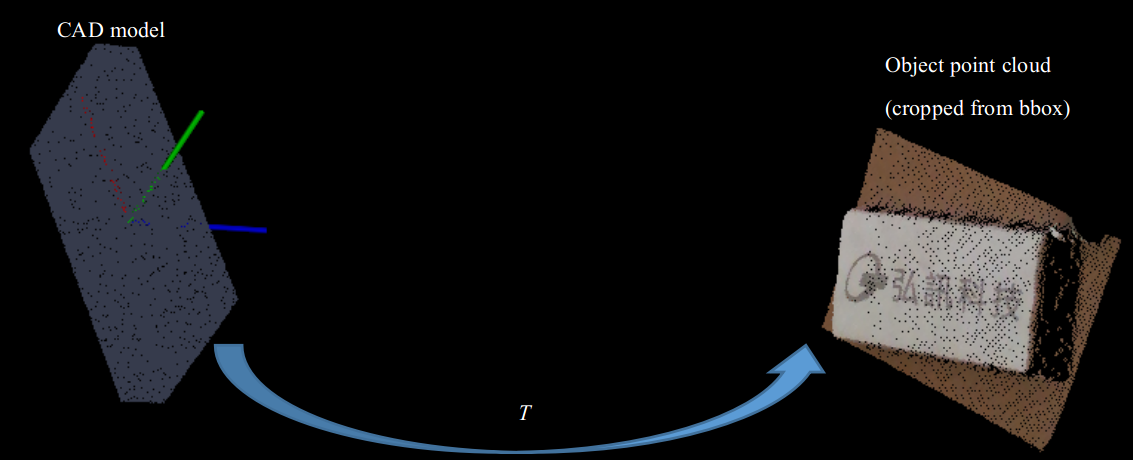
\includegraphics[width=14cm]{match_diagram}
  \caption{位姿估计示意图}
  \label{fig:match_diagram}
\end{figure}

相机所采集到的目标点云是一组包含空间三维坐标(x,y,z)以及颜色(r,g,b)的点集\footnote{对点集(point set)与点云(point cloud)不做区分,都指包含坐标点的集合},由于此处并不需要颜色信息,因此对目标点云只保留空间位置信息,去除颜色信息后的目标点云记为点集$P$。三维模型亦可通过采样得到一组包含空间三维坐标的点集,记为$Q$。A4PCS-ICP算法就可以简化为求解一个刚体变换$T$使得点集$P$中的点经过矩阵$T$变换后,尽可能与点集$Q$重合。更为准确地,A4PCS-ICP算法就可以简化为求解一个LCP(Largest Common Pointset)问题:

{\kai LCP问题:给定两个点集$P$和$Q$,在给定距离误差$\delta$下,求解点集$P$的最大子集$P'$,使得$T(P')$和点集$Q$之间的距离在合适的距离度量下小于$\delta$,其中$T$是一个刚体变换。}

\subsection{背景介绍}
LCP问题并不是一个新的问题,解决该问题的算法也有很多,尤其是近些年来,随着几何扫描相关技术的发展,如何将多次扫描或者多个设备采集的三维信息统一到一个坐标系下成为研究的热点,其本质上可以归结为LCP问题或其衍生问题,这些问题是计算机几何学和计算机视觉中的基础问题。

其中一个比较流行的算法是通过使用稳定的局部几何描述子来匹配得到粗略的刚体变换,然后紧接着使用ICP算法迭代获取较为精确的刚体变换\cite{li2005multiscale}。这种算法的效果十分取决于所选取的描述子,通常一般的描述子对传感器噪声都比较敏感,尤其是一些低精度的传感器,常用的局部几何特征描述子有SHOT\cite{salti2014shot}、FFPH\cite{rusu2009fast}等;还有一种比较流行的方法是通过几何希哈方法从事先设置好的候选集中来选择合适的刚体变换\cite{wolfson1997geometric};一些随机算法,如RANSAC(Random Sample Consesue)\cite{bolles1981ransac}通常需要足够长的时间才能保证得到合适的解。

上述介绍的一些算法,有些对噪声的鲁棒性不强,有些时间复杂度极高,有些也难以处理部分重叠的情况,即点集$P$和$Q$之间只有一部分点集是相匹配的,因此难以实际直接应用到本文所需要解决的问题,其效果也难以让人满意。对此,本文基于4PCS(4-Points Congruent Sets)算法设计了有效解决点云匹配的算法A4PCS-ICP。

\section{A4PCS-ICP算法}
\subsection{算法框架}
A4PCS-ICP算法基于4PCS,针对4PCS的瓶颈,有效地降低了其时间复杂度,然后通过与ICP算法配合提高匹配的精度,其整体框架如图~\ref{fig:4pcs-pe}~所示。
\begin{figure}[ht]
  \centering
  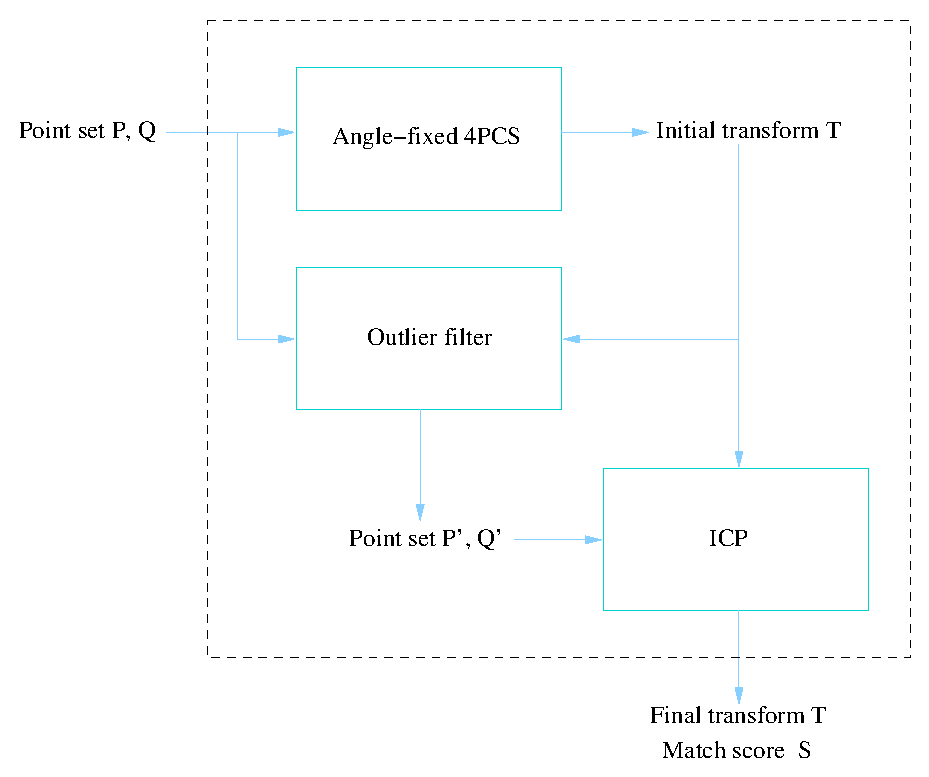
\includegraphics[width=12cm]{4pcs-pe}
  \caption{A4PCS-ICP算法框架}
  \label{fig:4pcs-pe}
\end{figure}
A4PCS-ICP由三个模块组成:Angle-fixed 4PCS、Outlier filter和ICP,Angle-fixed 4PCS是4PCS算法的优化版,也是A4PCS-ICP算法的核心,根据输入的两个点集,输出两个点集之间的粗略的变换关系;Outlier filter根据Angle-fixed 4PCS的输出对点集$P'$和$Q'$进行滤波,去掉一些离群点,用以提高下一步ICP算法的精度;ICP模块通过以Angle-fixed filter输出的变换关系为初始值对滤波后的两个点集进行迭代求解最佳的刚体变换关系,输出最终的变换关系$T$,也是目标的位姿。

\subsection{Angle-fixed 4PCS算法}
介绍Angle-fixed 4PCS算法之前,首先先详细介绍一下4PCS算法,4PCS算法是一个对3D点集全局匹配的算法,即使所给的两个3D点集有小的重叠,4PCS都能给出较好的结果,并且对噪声有一定的鲁棒性。这种方法对初始位姿没有任何要求,其核心是从3D点集中提取出所有与给定平面4-points近似全等的共面4-points,该算法时间复杂度为$O(n^2+k)$,其中$n$是3D点集中点的个数,$k$是提取出的4-points个数。4PCS使用十分广泛,并且引申出许多相关的变种\cite{corsini2013fully}。

\begin{algorithm}
  \caption{4PCS算法}
  \label{alg:4pcs}
  \KwIn{Point sets $P$ and $Q$, measure level $\delta$}
  \KwOut{Rigid transform $T$}
  $h\leftarrow 0$\;
  \For {$i = 1$ to $L$} {
    $B\leftarrow$ SELECTCOPLANARBASE($P$)\;
    $U\leftarrow$ FINDCONGRUENT($B,Q,\delta$)\;
    \ForAll {4-points coplannar sets $U_i\in U$} {
      $T_i\leftarrow$ best rigid transform that aligns $B$ to $U_i$ in the least square sense\;
      Find $S_i\subseteq P$, such that $d(T_i(S_i), Q)\leq\delta$\;
    }
    $k\leftarrow arg\;\underset{i}{max}\left\{|S_i|\right\}$\;
    \If {$|S_k| > h$} {
      $h\leftarrow |S_k|$\;
      $T\leftarrow T_k$\;
    }
    \Return $T$\;
  }
  \BlankLine
  \BlankLine
  \BlankLine
  \BlankLine
  \SetKwProg{Def}{def}{:}{}
  \Def{FINDCONGRUENT($B\equiv\left\{\mathbf{b_1},\mathbf{b_2},\mathbf{b_3},\mathbf{b_4}\right\},Q,\delta)$} {
    $d_1\leftarrow\;\parallel\mathbf{b_1}-\mathbf{b_2}\parallel$\;
    $d_2\leftarrow\;\parallel\mathbf{b_3}-\mathbf{b_4}\parallel$\;
    计算$R_1\equiv\left\{(\mathbf{p}_i,\mathbf{p}_j)\;|\;\mathbf{p}_i,\mathbf{p}_j\;\in Q\right\}$,使得$\parallel\mathbf{p}_i-\mathbf{p}_j\parallel\;\in [d_1-\delta,d_1+\delta]$\;
    计算$R_2\equiv\left\{(\mathbf{p}_i,\mathbf{p}_j)\;|\;\mathbf{p}_i,\mathbf{p}_j\;\in Q\right\}$,使得$\parallel\mathbf{p}_i-\mathbf{p}_j\parallel\;\in [d_2-\delta,d_2+\delta]$\;
    \ForAll {$r_{1i}\in R_1$} {
      计算与定量$r_1$和$r_2$相关的四个点$\left\{\mathbf{e}_{1i}^1,\mathbf{e}_{1i}^2,\mathbf{e}_{1i}^3,\mathbf{e}_{1i}^4\right\}$,记$\Pi(\mathbf{e}_{1i}^j)=r_{1i}$\;
    }
    对点集$\left\{\mathbf{e}_{1i}^j\right\}$在$\mathbb{R}^3$空间建立range tree的数据结构\;
    \ForAll {$r_{2i}\in R_1$} {
      计算与定量$r_1$和$r_2$相关的四个点$\left\{\mathbf{e}_{2i}^1,\mathbf{e}_{2i}^2,\mathbf{e}_{2i}^3,\mathbf{e}_{2i}^4\right\}$,记$\Pi(\mathbf{e}_{1i}^j)=r_{1i}$\;
    }
    $U'\leftarrow\varnothing$\;
    \ForAll {$\mathbf{e}_{2i}^j$} {
      在range tree中以$\delta$为领域检索点$\mathbf{e}_{2i}^j$附近的点,对于每个检索到的点$\mathbf{q}$,建立与$B$相对应的4个点的点集$U'\leftarrow\left\{U',(\Pi(\mathbf{q}),\Pi(\mathbf{e}_{2i}^j))\right\}$\;
    }
    \Return $U'$\;
  }
\end{algorithm}

{\kai 4PCS算法流程}:算法流程如\ref{alg:4pcs}所示,该算法输入两个点集$P$和$Q$,还有距离参数$\delta$,返回两个点集之间的刚体变换$T$。4PCS基于以下事实:{\kai 共面点集中定义的比例在仿射变换,包括刚体运动中保持不变。}举例来说,定义点集$X:=\left\{\mathbf{a},\mathbf{b},\mathbf{c},\mathbf{d}\right\}$,其中4个点不都在同一条直线上,设直线$ab$和$cd$相交于点$\mathbf{e}$,定义两个比例:
\begin{equation}
  \begin{array}{ccc}
    r_1& =& {\parallel \mathbf{a}-\mathbf{e}\parallel}/{\parallel \mathbf{a}-\mathbf{b}\parallel}\\
    r_2& =& {\parallel \mathbf{c}-\mathbf{e}\parallel}/{\parallel \mathbf{c}-\mathbf{d}\parallel}
  \end{array}
\end{equation}
则在仿射变换下所定义的$r_1$和$r_2$均保持不变,如图\ref{fig:4points}。
\begin{figure}[ht]
  \centering
  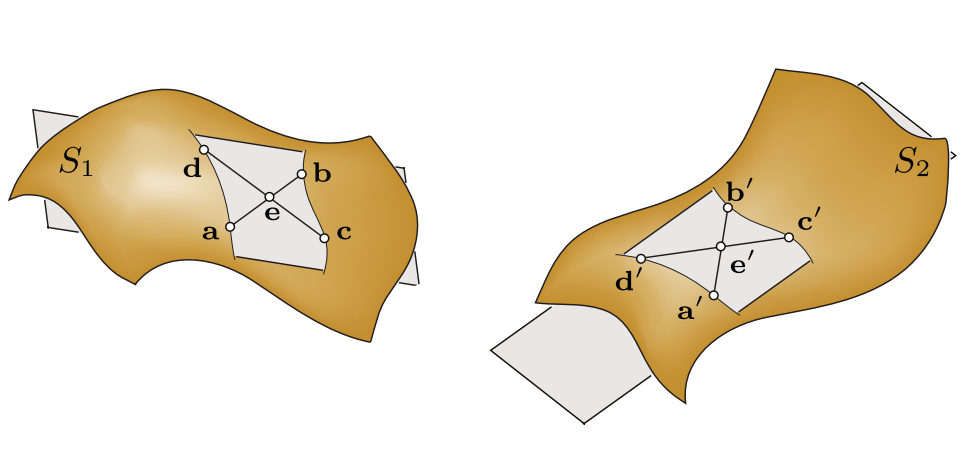
\includegraphics[width=12cm]{4points}
  \caption{4-points比例的仿射不变性}
  \label{fig:4points}
\end{figure}
如果曲面$S_1$和$S_2$匹配,并且4-points共面基在重叠区域,则$\mathbf{a},\mathbf{b},\mathbf{c},\mathbf{d}$对应的四个点$\mathbf{a}',\mathbf{b}',\mathbf{c}',\mathbf{d}'$也共面,并且
\begin{equation}
  \begin{array}{ccc}
    {\parallel \mathbf{a}'-\mathbf{e}'\parallel}/{\parallel \mathbf{a}'-\mathbf{b}'\parallel}&=&r_1\\
    {\parallel \mathbf{c}'-\mathbf{e}'\parallel}/{\parallel \mathbf{c}'-\mathbf{d}'\parallel}&=&r_2\\
  \end{array}
\end{equation}


4PCS算法另一个关键技术是使用了{\kai 宽基}(\emph{wide-base}),相比于一般的基,宽基中基的长度更长,如图\ref{fig:wide-base}所示,图片上半部分是使用宽基匹配的曲线,图片下半部分是使用一般的基匹配的曲线,显然,通过比较可以发现宽基相比普通基有更稳定的匹配结果,相关理论证明见文献\cite{goodrich1994practical}。
\begin{figure}[ht]
  \centering
  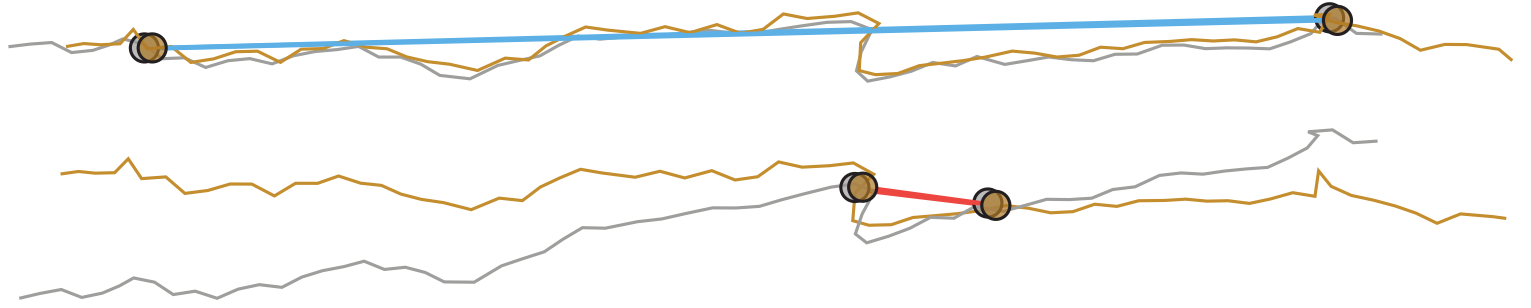
\includegraphics[width=14cm]{wide-base}
  \caption{宽基的匹配稳定性}
  \label{fig:wide-base}
\end{figure}

回到4PCS算法具体实现,算法的主体其实是一个RANSAC循环,每次循环首先会从点集$P$中挑选共面的宽基$B$,具体实现时,先从点集$P$中随机选取3个点,然后在剩下的点中选取第四个点构成共面的四点,第四个点的选取尽可能使得每个点之间的距离最大(因为我们要使用宽基),并且与前3个点近似共面(显然由于噪声的存在,完全共面并不现实),但如果第四个点选取的过远也会出现问题,因为如果宽基超过两个点集的重叠区域则难以匹配,因此当选以最大距离取宽基造成误差变大时以$f=1,0.5,0.25,\ldots$的比率降低最大距离来选取宽基。

在点集$P$中选取好宽基$B$后,算法下一步会在点集$Q$中通过4-points的仿射不变性找出所有与宽基$B$“全等”的基,构成集合$U$。在$Q$中选取基的方法见算法\ref{alg:4pcs}中的FINDCONGRUENT函数,函数首先使用基$B$中的点先定义两个仿射无关的比例,如图\ref{fig:findbase}中左边的图所示。
\begin{figure}[ht]
  \centering
  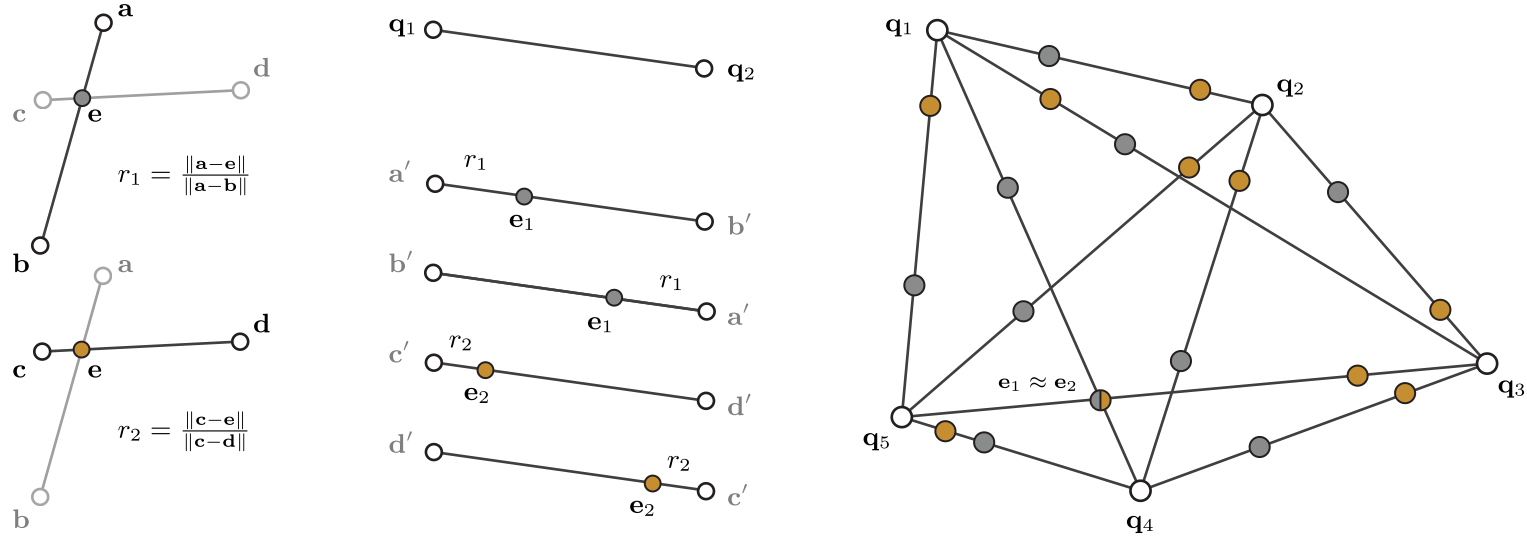
\includegraphics[width=15cm]{findbase}
  \caption{寻找近似“全等”的基示意图}
  \label{fig:findbase}
\end{figure}
假设在点集$Q$中找到两点$\mathbf{q}_1$和$\mathbf{q}_2$,并且$\left|\parallel \mathbf{q}_1-\mathbf{q}_2\parallel - \parallel \mathbf{a}-\mathbf{b}\parallel\right| \leq \delta$,则点$\mathbf{q}_1,\mathbf{q}_2$有可能与点$\mathbf{a}, \mathbf{b}$对应,则直线$\mathbf{a}\mathbf{b}$与$\mathbf{c}\mathbf{d}$相交的点$\mathbf{e}$的对应点可能为
\begin{equation}
  \mathbf{e}_1 = \mathbf{q}_1 + r1(\mathbf{q}_2-\mathbf{q}_1)
\end{equation}
或者
\begin{equation}
  \mathbf{e}_1 = \mathbf{q}_2 + r1(\mathbf{q}_1-\mathbf{q}_2)
\end{equation}
同理也可以根据$\mathbf{c},\mathbf{d}$的对应点(设为$\mathbf{q}_3, \mathbf{q}_4$)求得$\mathbf{e}$的对应点
\begin{equation}
  \mathbf{e}_2 = \mathbf{q}_3 + r1(\mathbf{q}_4-\mathbf{q}_3)
\end{equation}
或者
\begin{equation}
  \mathbf{e}_2 = \mathbf{q}_4 + r1(\mathbf{q}_3-\mathbf{q}_4)
\end{equation}
则当$\mathbf{e}_1\approx \mathbf{e}_2$时,$\mathbf{q}_1,\mathbf{q}_2,\mathbf{q}_3,\mathbf{q}_4$就是我们所要找的一组与点$\mathbf{a},\mathbf{b},\mathbf{c},\mathbf{d}$近似“全等”的基,如图\ref{fig:findbase}中右边图中的$\mathbf{q}_5,\mathbf{q}_3,\mathbf{q}_4,\mathbf{q}_1$。

具体实现时,当我们在点集$Q$中找出了所有可能的$\mathbf{e}_1$和$\mathbf{e}_2$后,找出其中近似相等的$\mathbf{e}_1$和$\mathbf{e}_2$可以通过range树\cite{arya1998optimal}来实现,对于大小为$n$的点集,range树的建立时间复杂度为$O(n\lg n)$,查询附近点的时间复杂度为$O(\lg n + k)$,其中$k$是查询到点的个数。

在$Q$中找出所有与基$B$近似“全等”的基后,下一步就是计算出最优的刚体变换$T$。对于$U$中的每个基$U_i$,我们可以利用最小二乘\cite{horn1987closed}的思想计算$B$到$U_i$的刚体变换$T_i$。得到刚体变换$T_i$后,我们将点集$P$进行变换$T_i$,然后对变换后的点集中的点在$Q$中查找最近点,统计最近点距离小于$\delta$的个数$S_i$,$S_i$也是评价$T_i$效果的分数,分数越高的$T_i$就是我们要求的最优刚体变换$T$。

{\kai 4PCS算法时间复杂度:}设输入的两个点集$P,Q$的大小分别为$m,n$。算法中最耗时的部分是FINDCONGRUENT函数:从点集$Q$中选取距离为$d_1$和$d_2$的点对,其时间复杂度为$O(n^21)$,然后建立和查询range树,其复杂度为$O(n^2+k$,其中$k$是满足条件的基个数,因此4PCS算法整体的时间复杂度为$O(n^2+k)$,空间复杂度显然为$O(n)$。

{\kai 4PCS算法不足:}仔细研究4PCS算法,可以发现从点集$Q$中提取的基与$B$并不是全等的,如图\ref{fig:4pcs-flaw}所示,
\begin{figure}[ht]
  \centering
  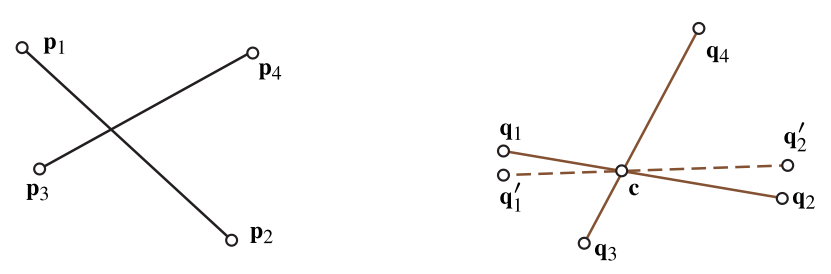
\includegraphics[width=12cm]{4pcs-flaw}
  \caption{4PCS中"全等“的基}
  \label{fig:4pcs-flaw}
\end{figure}
将线段$\mathbf{q}_1\mathbf{q}_2$绕交点转动一定角度后便不再与原基全等,但是4PCS仍然会找出点$\mathbf{q}_1',\mathbf{q}_2',\mathbf{q}_3,\mathbf{q}_4$作为与$\mathbf{p}_1',\mathbf{p}_2',\mathbf{p}_3,\mathbf{p}_4$全等的基。这一缺点会导致4PCS算法需要更多的求解时间,并且还有可能影响最终的匹配结果。

@todo: 4pcs算法改进

\subsection{Outlier filter}
从图~\ref{fig:match_diagram}其实可以看出目标点云有许多点并不属于目标物体,尤其是检测结果没有mask只能使用bbox分割目标时,不属于目标物体的离群点就尤其的多。因此,为了提高最终的匹配精度,除去这些离群点十分有必要,Outlier filter模块的作用就是根据Angle-fixed 4PCS输出的初始刚体变换来去除点云数据中的离群点,从而提升下一步ICP算法匹配的精度,使最终估计的位姿精度提高。

Outlier filter模块的核心算法如算法\ref{alg:outlier-filter}所示。
\begin{algorithm}[ht]
  \caption{Outlier filter算法}
  \label{alg:outlier-filter}
  \KwIn{Point sets $P$ and $Q$, Initial transform $T$, Distance tolerance $\delta$}
  \KwOut{Point sets $P'$ and $Q'$}
  $P'\leftarrow P$\;
  $Q'\leftarrow \varnothing$\;
  \ForAll {point $\mathbf{p}_i\in P$} {
    $\mathbf{p}_i\leftarrow T(\mathbf{p}_i)$\;
  }
  对点集$P$在$\mathbb{R}^3$空间建立kd树的数据结构\;
  \ForAll {point $\mathbf{q}_i\in Q$} {
    在kd树中检索出距离点$\mathbf{q}_i$最近的点$\mathbf{p}$\;
    $d\leftarrow\;\parallel\mathbf{q}_i-\mathbf{p}\parallel$\;
    \If {$d \leq \delta$} {
      $Q'\leftarrow \left\{Q', \mathbf{q}_i\right\}$\;
    }
  }
  \Return $P'$,$Q'$\;
\end{algorithm}
算法输入点集$P$和$Q$,需要参数初始刚体变换$T$,以及允许的距离误差$\delta$,由于点集$P$是由物体的CAD模型转换过来的,因此不对其进行滤波,只对点集$Q$进行离群点去除。具体方法是,首先使用$T$对点集$P$进行刚体变换;然后对变换后的点集建立kd树,建立kd树的目的是为了快速在点集$P$中找到距离某点最近的点,其查找的时间复杂度为$O(kN^{1-1/k}$,其中$k$是所建立kd树的维数,显然对于三维空间中点集为3,$N$是建立的kd树的节点个数;建立好kd树后,对点集$Q$中的每个点在kd树中找到与之距离最近的点,如果两点间的距离大于所设的参数$\delta$,则在点集Q中去除该点。实际运行Outlier filter算法的效果如图\ref{fig:outlier-filter}所示。
\begin{figure}[ht]
  \centering
  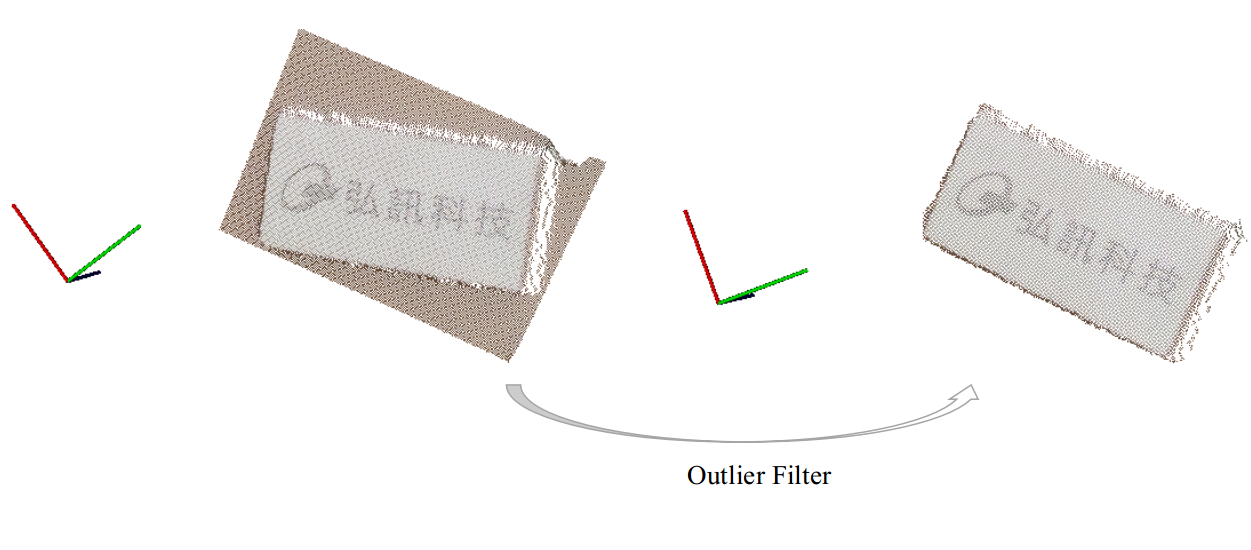
\includegraphics[width=13cm]{outlier-filter}
  \caption{Outlier filter效果图}
  \label{fig:outlier-filter}
\end{figure}


\subsection{ICP算法}
ICP(Iterative Closest Point)算法,即最近点迭代算法,是最为经典的数据配准算法。ICP算法本质上是基于最小二乘法的最优配准方法。该算法重复进行选择对应关系点对,计算最优刚体变换,直到满足正确配准的收敛精度要求。由于ICP算法是一种迭代算法,因此只要时间允许便可以获取足够精度的解,但也正因为如此,ICP也容易陷入局部最优解。本文充分考虑了ICP算法的这个特点,通过Angle-fixed 4PCS算法给出初始的刚体变换来避免ICP算法陷入局部最优解,同时通过迭代来提高最后输出的刚体变换精度。下面介绍一下ICP算法的基本原理。

给定两个点集$P_n:=\left\{\mathbf{p}_1,\mathbf{p}_2,\ldots,\mathbf{p}_n\right\}$和$Q_m:=\left\{\mathbf{q}_1,\mathbf{q}_2,\ldots,\mathbf{q}_m\right\}$,以及初始旋转变换$R$和平移变换$t$,以及迭代结束额距离误差$\delta$,ICP算法迭代步骤如下:
\begin{itemize}
\item {\kai 步骤1:}根据当前$R$和$t$,对于点集$P_n$中的每个点在$Q_m$中找出距离最近的点,构成点集$Q_n$;
\item {\kai 步骤2:}计算$P_n$和$Q_n$之间的距离的均方根误差:
  \begin{equation}
    E(R,t) = \frac{1}{n}\sum_{i=1}^n{\parallel \mathbf{q}_i - R\mathbf{p}_i - t\parallel}
  \end{equation}
  通过奇异值分解求得使得$E(R,t)$最小的$R'$和$t'$;
\item {\kai 步骤3:}如果$E(R,t) < \delta$,结束迭代;否则$R\leftarrow R'$,$t\leftarrow t'$,跳转至步骤1。
\end{itemize}

ICP算法的迭代过程还是相对来说十分简单的,唯一需要思考一下的是如何求得最小化$E(R,t)$的$R'$和$t'$,通过奇异值分解求解$R'$和$t'$的方法如下:

首先,记
\begin{equation}
  \left\{
  \begin{array}{ccccc}
  P_n'& = &\left\{\mathbf{p}_i-\mathbf{\mu}_p \;|\; \forall \mathbf{p}_i \in P_n\right\}&:=&\left\{\mathbf{p}'_i\right\}\\
  Q_n'& = &\left\{\mathbf{q}_i-\mathbf{\mu}_q \;|\; \forall \mathbf{q}_i \in Q_n\right\}&:=&\left\{\mathbf{q}'_i\right\}
  \end{array}
  \right.
\end{equation}
其中
\begin{equation}
  \left\{
    \begin{array}{ccc}
      \mathbf{\mu}_p&=&\frac{1}{n}\sum_{i=1}^n{\mathbf{p}_i}\\
      \mathbf{\mu}_q&=&\frac{1}{n}\sum_{i=1}^n{\mathbf{q}_i}
    \end{array}
  \right.
\end{equation}
再另
\begin{equation}
  W = \sum_{i=1}^n{\mathbf{p}_i'\mathbf{q}_i'}
\end{equation}
然后对矩阵$W$进行奇异值分解:
\begin{equation}
  W = U\Sigma V^T
\end{equation}
则
\begin{equation}
  \left\{
    \begin{array}{ccc}
      R'&=&UV^T \\
        t'&=&\mathbf{\mu}_p-R'\mathbf{\mu}_q
    \end{array}
    \right.
\end{equation}

\section{点云匹配实验}
为了评价所设计的算法A4PCS-ICP,考察其匹配精度以及时间性能,本文设计了位姿估计的实验,不但考察了A4PCS-ICP的性能,还与其他一些算法作比较,验证了A4PCS-ICP算法的匹配的精确度。

@todo: 点云匹配实验

\section{本章小结}
@todo: matcher 小结

%%% Local Variables:
%%% TeX-master: "../thesis.tex"
%%% End:
%!TEX root = ../thesis.tex
\chapter{实验验证}
\label{chap:experiment}
%!TEX root = ../thesis.tex
\chapter{结论与展望}
\label{conclusion}

\section{结论}

\section{进一步工作的方向}




%%% 其它部分
\backmatter

\makeatother

% 致谢
\begin{ack}\fs
  % TODO
逾尺的札记和研究纪录凝聚成这么薄薄的一本,高兴和欣慰之余,不禁感慨系之。记得鲁迅在一篇文章里写道:“人类的奋战前行的历史,正如煤的形成,当时用大量的木材,结果却只是一小块”。倘若这一小块有点意义的话,则是我读书生活的最好纪念,也令我对于即将迈入的新生活更加充满信心。
回想读书生活,已经整整二十个年头,到同济求学将近五年,攻读博士学位也已三年了。进入同济大学以来,深深醉心于一流学府的大家风范。名师巨擘,各具特点;中西融合,文质相顾。处如此佳境以陶铸自我,实乃人生幸事。

\ackdate
\end{ack}

%%% Local Variables:
%%% TeX-master: "../thesis.tex"
%%% End:

%%% 参考文献
\bibliographystyle{tongjibib-lxd}
\bibliography{ref/ref}

% 附录
\begin{appendix}
\chapter{补充资料}
\label{Appendix}
@todo:可能需要补充的内容……


%%% Local Variables:
%%% TeX-master: "../thesis.tex"
%%% End:
\end{appendix}

%%% 个人简历
\begin{resume}
% \chapter{个人简历、在读期间发表的学术论文与研究成果}

\resumeitem{个人简历}
\hskip-0.81cm 李勇奇,男,1992年12月生。
\\
2015年6月毕业于南京理工大学 自动化专业 获工学学士学位。
\\
2015年9月入同济大学攻读控制科学与工程专业的硕士学位。

% \resumeitem{已发表论文}
% \hskip-0.81cm [1] XU, Jing, Chenxiao CAI, Yongqi LI, and Y. Zou. "Dual-loop path tracking and control for quad-rotor miniature unmanned aerial vehicles." Control Theory \& Applications 32, no. 10 (2015): 1335-1342.
% \begin{enumerate}[{[}1{]}]
%   \item XU, Jing, Chenxiao CAI, Yongqi LI, and Y. Zou. "Dual-loop path tracking and control for quad-rotor miniature unmanned aerial vehicles." Control Theory \& Applications 32, no. 10 (2015): 1335-1342.
% \end{enumerate}

	% \resumeitem{已获得专利}
	% \begin{enumerate}[{[}1{]}]
	% \item ...
	% \item ...
	% \end{enumerate}

\resumeitem{科研竞赛获奖}
\hskip-0.81cm [1] 2016 RoboCup机器人世界杯标准平台组八强,莱比锡,德国

\hskip-0.81cm [2] 2016 RoboCup 机器人世界杯中国赛标准平台组冠军,安徽,中国

% \begin{enumerate}[{[}1{]}]
%   \item \hs2016 RoboCup机器人世界杯标准平台组八强,莱比锡,德国
%   \item 2016 RoboCup 机器人世界杯中国赛标准平台组冠军,安徽,中国
% \end{enumerate}

\end{resume}

%%% Local Variables:
%%% TeX-master: "../thesis.tex"
%%% End:

\end{document}
